\documentclass[12pt,a4paper]{article}

% Font and language setup
\usepackage{fontspec}
\usepackage{polyglossia}
\setmainlanguage{polish}
\setotherlanguage{english}

\usepackage{microtype}
\usepackage[margin=2.5cm]{geometry}
\usepackage{setspace}
\usepackage{booktabs}
\usepackage{array}
\usepackage{longtable}
\usepackage{siunitx}
\usepackage{amsmath}
\usepackage{amssymb}
\usepackage{graphicx}
\usepackage{float}
\usepackage{tabularx}
\usepackage{pdflscape}
\usepackage{titlesec}
\usepackage{fancyhdr}
\usepackage{url}
\usepackage{hyperref}
\usepackage[backend=bibtex,style=authoryear,sorting=nyt,maxcitenames=2,maxbibnames=99]{biblatex}

\onehalfspacing
\setlength{\parindent}{1.25cm}
\setlength{\parskip}{0.15\baselineskip}
\setlength{\headheight}{14pt}
\setcounter{tocdepth}{2}
\setcounter{secnumdepth}{2}
\emergencystretch=3em
\sisetup{
  output-decimal-marker = {,},
  group-separator = { },
  detect-all
}
\newcolumntype{L}[1]{>{\raggedright\arraybackslash}p{#1}}
\newcolumntype{C}[1]{>{\centering\arraybackslash}p{#1}}

\addbibresource{references.bib}

\hypersetup{
  colorlinks=true,
  linkcolor=black,
  citecolor=black,
  urlcolor=blue
}

\titleformat{\section}{\large\bfseries}{\thesection.}{0.5em}{}
\titleformat{\subsection}{\normalsize\bfseries}{\thesubsection.}{0.5em}{}
\newcommand{\sectionbreak}{\clearpage}

\pagestyle{fancy}
\fancyhf{}
\fancyhead[L]{\small BDP jako warunkowy katalizator automatyzacji}
\fancyhead[R]{\small\thepage}
\renewcommand{\headrulewidth}{0.4pt}

\newcommand{\amor}{\texorpdfstring{\href{https://github.com/boombustgroup/amor-fati}{\textit{amor-fati}}}{amor-fati}}
\newcommand{\ledger}{\texorpdfstring{\href{https://github.com/boombustgroup/amor-fati-ledger}{\texttt{amor-fati-ledger}}}{amor-fati-ledger}}
\newcommand{\bbg}{\texorpdfstring{\href{https://boombustgroup.com/}{BoomBustGroup}}{BoomBustGroup}}
\newcommand{\bdp}{BDP}
\newcommand{\ubi}{UBI}

\title{BDP jako warunkowy katalizator automatyzacji:\\
od równowagi DSGE do wykonywalnego modelu SFC-ABM gospodarki polskiej}
\author{Mateusz Maciaszek\\MBA - Ekonomia Menedżerska}
\date{Wersja robocza, \today}

\begin{document}

\maketitle

\begin{abstract}
Niniejsza praca analizuje Bezwarunkowy Dochód Podstawowy nie tylko jako instrument redystrybucyjny, lecz jako potencjalny szok menedżerski wpływający na koszt pracy, koszt kapitału, popyt, bilanse firm oraz decyzje o automatyzacji. Punktem odniesienia jest raport Międzynarodowego Funduszu Walutowego \textit{Fiscal Monitor: Tackling Inequality} z 2017 r., który ujmuje BDP w modelu DSGE dla Stanów Zjednoczonych oraz w analizie statycznej dla Polski opartej na danych LIS 2013. Praca argumentuje, że pytanie menedżerskie dotyczy nie tylko nowej równowagi, lecz przede wszystkim ścieżki przejścia: czy firmy mają płynność, marże, kredyt i warunki popytowe, aby sfinansować reakcję technologiczną. Wykorzystano w tym celu \amor{}, wykonywalny model stock-flow consistent agent-based polskiej gospodarki. Eksperyment dotyczy deficytowo finansowanego BDP w horyzoncie 60 miesięcy i 10 seedów. W wariancie centralnym \(\lambda = 0{,}5\) BDP nie działa jako liniowy akcelerator automatyzacji. Efekt jest warunkowy: adopcja AI/hybrid rośnie do okolic scenariusza \texttt{--bdp 2000}, po czym spada, gdy kanał fiskalno-finansowy zaczyna ograniczać zdolność inwestycyjną sektora prywatnego. Warianty finansowania przez podatki lub cięcia wydatków nie są przedmiotem tego eksperymentu i mogą zmienić wielkość oraz kierunek efektu.

\medskip
\noindent\textbf{Słowa kluczowe:} Bezwarunkowy Dochód Podstawowy, BDP, UBI, SFC-ABM, modele agentowe, DSGE, automatyzacja, koszt kapitału, płaca rezerwowa, polityka pieniężna, gospodarka polska, ekonomia złożoności.

\medskip
\noindent\textbf{Kody JEL:} C63, D31, E17, E24, E52, H24, H53, O33.

\medskip
\noindent\textbf{Ujawnienie:} Silnik modelu \amor{} jest autorskim projektem open-source autora pracy, rozwijanym w ramach \bbg{}. Patch scenariusza BDP, dane Monte Carlo i skrypty replikacyjne są wydzielone do osobnego repozytorium pracy.

\medskip
\noindent\textbf{Kod i dane:} silnik modelu \amor{}; artefakty pracy, dane Monte Carlo i patch BDP w repozytorium \texttt{amor-fati-bdp-mba-paper}.
\newline
\noindent Base commit \amor{}: \path{2d8b46e5064abef9d7a054317028843837b6e1c4}; patch: \path{patches/amor-fati-bdp-scenario.patch}; dane: \path{mc/}.
\end{abstract}

\clearpage
\pdfbookmark[1]{Spis treści}{toc}
\tableofcontents
\clearpage

\section{Wprowadzenie: pytanie menedżerskie}

Decyzja inwestycyjna zarządu polskiej firmy w roku 2026 nie zapada w podręcznikowym stanie ogólnej równowagi. Zapada w środowisku, w którym wynagrodzenia, koszt finansowania, kurs PLN/EUR, ceny importowanych komponentów, dostępność kredytu i oczekiwania inflacyjne zmieniają się równocześnie. Dla zarządu i dyrektora finansowego pytanie o Bezwarunkowy Dochód Podstawowy nie jest więc wyłącznie pytaniem o redystrybucję. Jest pytaniem o marżę, płynność, inwestycje, strukturę kosztów i zdolność obsługi długu w kolejnych kwartałach po wprowadzeniu takiego programu.

W debacie publicznej BDP najczęściej występuje jako odpowiedź na automatyzację: skoro sztuczna inteligencja, robotyzacja i oprogramowanie wypierają część pracy, państwo powinno rozważyć dochód podstawowy jako zabezpieczenie społeczne \parencite{autor2015,brynjolfsson2014,acemoglu2018,acemoglu2020,graetzMichaels2018,freyOsborne2017,korinekStiglitz2019,susskind2020}. Taki kierunek rozumowania jest intuicyjny, ale jednostronny. Ta praca wychodzi od odwrotnej możliwości: BDP może nie tylko amortyzować skutki automatyzacji, lecz także zmieniać bodźce, które prowadzą firmy do automatyzacji. Innymi słowy, transfer publiczny może stać się jednym z mechanizmów przyspieszających substytucję pracy kapitałem.

Mechanizm ten nie jest jednak prosty. BDP może podnosić płacę rezerwową, czyli minimalny poziom wynagrodzenia, przy którym część gospodarstw domowych akceptuje zatrudnienie. To zwiększa presję kosztową po stronie firm. Równocześnie BDP zwiększa dochód gospodarstw domowych i może wspierać popyt, co poprawia warunki sprzedażowe przedsiębiorstw. Ten sam transfer powiększa jednak wydatki publiczne, deficyt i dług, a przez inflację, reakcję banku centralnego, rentowności obligacji, kurs walutowy i koszt długu korporacyjnego wpływa na koszt kapitału. Firma znajduje się więc między dwoma ruchami cen względnych: pracą, która może stać się droższa, oraz kapitałem, który także może stać się droższy.

Z tego powodu główne pytanie pracy nie brzmi: czy BDP jest dobry albo zły. Pytanie jest bardziej praktyczne: w jakim zakresie BDP może działać jako katalizator inwestycji w AI i automatyzację, a od którego momentu interakcja presji płacowo-rezerwowej oraz kanału fiskalno-finansowego zaczyna ograniczać zdolność firm do sfinansowania tej reakcji. Łączy ono makroekonomię z zarządzaniem, bo przekłada się na decyzje o długu, nakładach inwestycyjnych, technologii, zatrudnieniu i zabezpieczeniu ekspozycji walutowej.

Punktem odniesienia jest raport Międzynarodowego Funduszu Walutowego \textit{Fiscal Monitor: Tackling Inequality} z 2017 r. Raport MFW jest w tej pracy traktowany jako punkt odniesienia dla analizy redystrybucji, efektywności i dobrobytu w określonej ramie modelowej. W przypadku Polski wykorzystuje analizę statyczną opartą na danych LIS z 2013 r. To ujęcie pomaga zakotwiczyć skalę problemu, ale nie wyczerpuje problemu menedżerskiego. Dla firmy ważne jest nie tylko to, gdzie gospodarka może znaleźć się w nowej równowadze, lecz także to, co dzieje się po drodze: z płynnością, bilansem, kredytem, kursem walutowym, bankructwami, inwestycjami i heterogenicznymi reakcjami przedsiębiorstw.

Dlatego w pracy wykorzystano \amor{}, autorski wykonywalny model stock-flow consistent agent-based gospodarki polskiej rozwijany w ramach \bbg{}. Model jest skalibrowany do stanu Polski na 2026-04-30, a eksperyment BDP traktowany jest jako kontrfaktyczna ścieżka od tego punktu startowego. \amor{} nie opiera się na reprezentatywnym agencie: operuje na heterogenicznych gospodarstwach domowych, firmach, bankach, sektorze publicznym, banku centralnym i sektorze zewnętrznym. Każdy przepływ pieniężny w modelu musi mieć drugą stronę księgową. Hipoteza zostaje więc zapisana w mechanizmie, uruchomiona i porównana ze ścieżką bez BDP.

Wynik eksperymentu doprecyzowuje początkową intuicję. Mocna wersja hipotezy, zgodnie z którą wyższy BDP powinien prowadzić do coraz większej automatyzacji, nie znajduje potwierdzenia. W wariancie centralnym adopcja AI/hybrid rośnie do okolic scenariusza BDP 2000~PLN, po czym spada przy wyższych poziomach transferu. Oznacza to, że BDP może być katalizatorem automatyzacji tylko warunkowo: dopóki presja kosztowa i popytowa nie ograniczają zdolności sektora prywatnego do finansowania inwestycji. Dla zarządu próg absorpcji jest więc zmienną strategiczną: automatyzacja nie jest tylko wyborem technologicznym, lecz decyzją finansową podejmowaną pod ograniczeniem płynności, zadłużenia i ryzyka makroekonomicznego.

\section{Punkt odniesienia: MFW i modelowanie BDP}

Raport Międzynarodowego Funduszu Walutowego \textit{Fiscal Monitor: Tackling Inequality} analizuje BDP jako instrument redystrybucyjny, którego skutki należy oceniać przez koszty fiskalne, efektywność, wpływ na podaż pracy oraz zmianę nierówności \parencite{imf2017fiscal}. Szczególnie istotny jest Aneks 1.3, wykorzystujący dynamiczny stochastyczny model równowagi ogólnej zaadaptowany z pracy Lizarazo, Peralta-Alvy i Puya \parencite{lizarazo2017}.

W tej strukturze gospodarka jest podzielona na trzy sektory: sektor dóbr podlegających wymianie międzynarodowej, usługi wymagające niskich kwalifikacji oraz usługi wymagające wysokich kwalifikacji. Gospodarstwa domowe różnią się poziomem wykształcenia i są obarczone indywidualnymi szokami produktywności. Rynki pracy są segmentowane, a krajowe rynki kredytowe są niekompletne. Model porównuje wariant odniesienia z wariantami reform podatkowo-transferowych, w tym BDP finansowanym cięciami wydatków, wzrostem VAT lub wzrostem progresywnego PIT.

Wniosek MFW jest wewnętrznie spójny: BDP jest progresywny, ale przy tej samej skali kosztu fiskalnego może być zdominowany dobrobytowo przez instrumenty celowane, takie jak rozszerzenie Earned Income Tax Credit. W takim ujęciu pytanie brzmi: jaki instrument redystrybucyjny maksymalizuje dobrobyt społeczny przy zadanym koszcie i założonych mechanizmach finansowania?

Polska w raporcie MFW pojawia się w innej formule. Aneks 1.6 nie jest pełnym DSGE, lecz analizą częściowej równowagi statycznej (partial static equilibrium) opartą na danych Luxembourg Income Study dla Polski z 2013 r. Koszt brutto BDP skalibrowanego do 25\% mediany dochodu rynkowego po podatkach bezpośrednich na osobę wynosi 4,9\% PKB, redukcja współczynnika Giniego wynosi 0,04, redukcja stopy ubóstwa 6,9 punktu procentowego, a kwota BDP to 2 111 zł na osobę rocznie. Nominalnie odpowiada to około 176 zł na osobę miesięcznie, ale jest to wartość osadzona w danych z 2013 r. Po przybliżonej indeksacji rocznymi wskaźnikami CPI GUS za lata 2014--2025 daje to około 273 zł na osobę miesięcznie w cenach średniorocznych 2025 \parencite{gusCpiAnnual}. Właśnie dlatego nie należy porównywać nominalnych 176 zł bezpośrednio z poziomami siatki scenariuszy \amor{}, które są miesięcznym transferem na agenta reprezentującego gospodarstwo domowe w modelu skalibrowanym do Polski na 2026-04-30.

Most między MFW i \amor{} nie jest więc mapowaniem jeden do jednego. MFW Polska 2013 i \amor{} Polska 2026 odpowiadają na różne pytania, mają różne lata kalibracji i używają różnych jednostek transferu. Oryginalna kotwica fiskalna MFW, czyli 4,9\% PKB w roku kalibracji 2013, jest wartością historyczną dla tamtego ćwiczenia. Po indeksacji CPI kwota transferu wynosi około 273 zł na osobę miesięcznie; przy nominalnym PKB Polski 2025 z Article IV MFW daje to około 3,2\% PKB \parencite{imf2026polandArticleIV}. Tabela~\ref{tab:mfw-scale-bridge} pokazuje także pomocnicze odniesienie tej samej kwoty do wspólnego mianownika modelowego, czyli PKB wariantu bez BDP po 60 miesiącach w \amor{}; daje to około 2,32\% PKB. To nie jest scenariusz MFW ani wynik wariantu \amor{}, lecz przeliczenie pomostowe. Dlatego w dalszej interpretacji nie traktuję żadnego poziomu siatki jako dokładnej repliki MFW. BDP 500~PLN jest najbliższą kotwicą w ujęciu na osobę i kotwicą w porównywalnym mianowniku modelowym, a BDP 1000~PLN pozostaje blisko oryginalnej, historycznej kotwicy 4,9\% PKB z aneksu MFW.

Dla poziomów siatki \amor{} kolumna „Ekwiwalent na osobę” w tabeli~\ref{tab:mfw-scale-bridge} nie jest parametrem wejściowym modelu. Jest liczona jako dodatkowy miesięczny strumień transferów społecznych względem wariantu bez BDP, podzielony przez populację referencyjną 38 mln osób. Dlatego poziom BDP 500~PLN na agenta reprezentującego gospodarstwo domowe odpowiada około 283 PLN/os./mies., a nie 500 PLN/os./mies.

\begin{table}[htbp]
\centering
\scriptsize
\caption{Skala polskiego wariantu MFW względem siatki eksperymentu \amor{}}
\label{tab:mfw-scale-bridge}
\begin{tabularx}{\textwidth}{@{}p{0.20\textwidth}rrrX@{}}
\toprule
Pozycja & Ekwiwalent na osobę & Koszt wg źródła & Koszt porównawczy & Interpretacja \\
 & PLN/os./mies. & \% PKB źródła & \% PKB bez BDP, m60 & \\
\midrule
MFW, Polska, ceny 2013 & 176 & 4,9 & -- & kwota MFW: 2 111 PLN/os./rok; mianownik PKB 2013 \\
MFW, Polska, ceny 2025 & 273 & 3,2 & 2,32 & kwota MFW po CPI; kolumna 4 to tylko wspólny mianownik modelu \\
BDP 500~PLN & 283 & -- & 2,40 & poziom siatki najbliższy MFW po CPI \\
BDP 1000~PLN & 565 & -- & 4,80 & blisko historycznej kotwicy 4,9\% PKB MFW \\
BDP 2000~PLN & 1 130 & -- & 9,59 & lokalny szczyt adopcji AI/hybrid w wariancie centralnym \\
BDP 3000~PLN & 1 700 & -- & 14,42 & wysoki impuls fiskalno-finansowy \\
\bottomrule
\end{tabularx}
\end{table}


Tabela~\ref{tab:mfw-scale-bridge} rozdziela dwa mianowniki: koszt w źródle oraz koszt przeliczony na wspólny mianownik modelowego PKB wariantu bez BDP po 60 miesiącach. Po takim rozdzieleniu widać, że polski wariant ilustracyjny MFW po indeksacji CPI znajduje się blisko najniższego dodatniego poziomu siatki \amor{} w ujęciu na osobę i w modelowym mianowniku PKB. Jednocześnie oryginalny koszt brutto MFW, liczony jako udział w PKB roku kalibracji 2013, pozostaje blisko scenariusza BDP 1000~PLN. Oznacza to, że most MFW--\amor{} ma charakter zakresu, a nie jednego punktu. Poziomy BDP od 1000 PLN do 3000 PLN testują coraz silniejsze impulsy fiskalno-dochodowe. Ich rolą nie jest odtworzenie polskiego ćwiczenia statycznego MFW, lecz przetestowanie progu, przy którym pozytywny impuls popytowy zaczyna ustępować interakcji presji płacowo-rezerwowej i ograniczeń fiskalno-finansowych.

\begin{table}[H]
\centering
\small
\caption{MFW i \amor{} jako komplementarne narzędzia analityczne}
\label{tab:mfw-vs-amor-fati}
\begin{tabularx}{\textwidth}{@{}L{0.20\textwidth}L{0.13\textwidth}>{\raggedright\arraybackslash}X@{}}
\toprule
Wymiar & Narzędzie & Ujęcie \\
\midrule
Pytanie badawcze & MFW & Jaki instrument redystrybucyjny poprawia równość i dobrobyt przy zadanym koszcie fiskalnym? \\
 & \amor{} & Jak BDP przechodzi przez bilanse, koszt kapitału, kurs, banki, inwestycje i decyzje firm o automatyzacji? \\
\addlinespace
Perspektywa czasu & MFW & Porównanie wariantów polityki w równowadze lub w analizie statycznej. \\
 & \amor{} & Ścieżka przejścia w horyzoncie 60 miesięcy. \\
\addlinespace
Jednostka BDP & MFW & Transfer na osobę, w polskim aneksie raportowany rocznie. \\
 & \amor{} & Miesięczny transfer na agenta reprezentującego gospodarstwo domowe, przeliczany następnie na ekwiwalent na osobę. \\
\addlinespace
Finansowanie & MFW & Warianty finansowania przez cięcia wydatków, VAT lub PIT; dla Polski koszt brutto w analizie statycznej. \\
 & \amor{} & Wariant deficytowy względem ścieżki bez BDP w \amor{}, z jawnym przejściem przez wydatki, deficyt i dług. \\
\addlinespace
Wyniki & MFW & Redystrybucja, ubóstwo, Gini, dobrobyt, koszt fiskalny. \\
 & \amor{} & Adopcja AI/hybrid, inwestycje, inflacja, stopa NBP, dług, deficyt, kurs, rachunek bieżący i bilanse banków. \\
\bottomrule
\end{tabularx}
\end{table}


Z perspektywy niniejszej pracy MFW nie jest przeciwnikiem, lecz punktem odniesienia. Raport odpowiada precyzyjnie na pytanie o redystrybucję i dobrobyt społeczny. \amor{} odpowiada na inne pytanie: czy firmy w trakcie przejścia mają finansową i organizacyjną zdolność do automatyzacji. To pytanie wymaga modelu, w którym ścieżka przejścia jest częścią wyniku.

\section{Luka analityczna: od stanu stałego do ścieżki przejścia}

Modele równowagi ogólnej są silne tam, gdzie pytanie dotyczy porównania uporządkowanych stanów gospodarki. Z perspektywy zarządu firmy problem BDP jest jednak problemem ścieżki. Firma nie inwestuje w punkcie terminalnym symulacji. Inwestuje w drugim, trzecim i czwartym roku transformacji, gdy nie zna jeszcze finalnego poziomu stóp procentowych, kursu walutowego, popytu, bankructw konkurentów ani własnej zdolności kredytowej.

Raport MFW nie modeluje kilku elementów kluczowych dla decyzji menedżerskiej w Polsce. Po pierwsze, nie opisuje endogenicznej substytucji pracy kapitałem w odpowiedzi na wzrost kosztu pracy i płacy rezerwowej. Po drugie, nie rozróżnia heterogenicznych firm o różnym poziomie marż, dźwigni, płynności i podatności na bankructwo. Po trzecie, nie wprowadza banków jako odrębnych podmiotów z ograniczeniami CAR, LCR, NSFR i portfelem NPL. Po czwarte, w polskim kontekście ważny jest sektor zewnętrzny: kurs PLN/EUR, importochłonność inwestycji, ceny importowane i rachunek bieżący.

Luka nie polega więc na tym, że DSGE jest złe. Luka polega na niedopasowaniu narzędzia do pytania. Jeżeli pytamy o welfare i redystrybucję w stanie równowagi, DSGE jest naturalnym instrumentem. Jeżeli pytamy o trajektorię firm, banków, budżetu państwa i kursu walutowego w trakcie przejścia, potrzebujemy modelu wykonującego przepływy bilansowe w czasie.

Z tego powodu niniejsza praca traktuje BDP jako szok przechodzący przez kilka kanałów transmisji jednocześnie: płacę rezerwową, popyt, inflację, politykę pieniężną, dług publiczny, sektor zewnętrzny, kredyt bankowy i decyzje inwestycyjne firm. W takim ujęciu wynik nie musi być monotoniczny. Ten sam transfer może wzmacniać popyt, ale jednocześnie zwiększać deficyt, koszt kapitału i presję na import.

\section{Hipoteza warunkowego przyspieszenia}

Hipotezę pracy można sformułować jako hipotezę warunkowego przyspieszenia automatyzacji. W ujęciu intuicyjnym brzmi ona następująco: instrument zaprojektowany jako osłona społeczna przed skutkami automatyzacji może sam zmienić ceny względne i warunki finansowania w taki sposób, że stanie się bodźcem do automatyzacji. Odwróceniu ulega zwyczajowy porządek przyczynowy. BDP nie jest wyłącznie skutkiem rozwoju AI; może być jednym z mechanizmów, które przyspieszają decyzje firm o zastępowaniu pracy kapitałem.

Ta hipoteza ma jednak dwie wersje. Wersja mocna jest monotoniczna: im wyższy BDP, tym silniejsza presja automatyzacyjna i tym większa adopcja AI/hybrid. Wersja słabsza, ale ekonomicznie bardziej realistyczna, jest warunkowa: deficytowo finansowany BDP może przyspieszać automatyzację tylko do momentu, w którym sektor prywatny zachowuje zdolność finansowania inwestycji. Po przekroczeniu pewnego progu ten sam transfer może ograniczać automatyzację nie dlatego, że sam wzrost długu mechanicznie wypiera nakłady inwestycyjne, lecz dlatego, że presja płacowo-rezerwowa tworzy potrzebę automatyzacji, a pogorszenie warunków fiskalno-finansowych zmniejsza przestrzeń bilansową firm do sfinansowania tej reakcji. Zakres tej pracy dotyczy właśnie wariantu deficytowego; finansowanie przez VAT, PIT, cięcia wydatków lub warianty mieszane mogłoby zmienić kanały transmisji.

Mikroekonomiczny komponent hipotezy opiera się na płacy rezerwowej. Jeżeli dochód niezależny od pracy rośnie, część gospodarstw domowych może wymagać wyższej płacy, aby zaakceptować zatrudnienie. Literatura teoretyczna i empiryczna dotycząca podatków, transferów oraz dochodu podstawowego nie wskazuje na jedną stabilną elastyczność podaży pracy; efekty zależą od konstrukcji programu, populacji i otoczenia rynku pracy \parencite{mirrlees1971,saez2002,vanParijs2017,forget2011,marinescu2018,kangas2019,jonesMarinescu2022,hoynesRothstein2019,banerjee2019}. Dlatego \(\lambda = 0{,}5\) należy traktować jako parametr scenariuszowy po stronie relatywnie silnego przełożenia transferu na płacę rezerwową, a nie jako bezpośrednią estymację empiryczną. W modelu \amor{} kanał ten jest zapisany jako:
\begin{equation}
  w^{res}_t = w^{min}_t + \lambda \cdot BDP,
\end{equation}
gdzie \(w^{res}_t\) oznacza płacę rezerwową, \(w^{min}_t\) płacę minimalną, a \(\lambda\) parametr przełożenia transferu na płacę rezerwową. W wariancie centralnym przyjęto \(\lambda = 0{,}5\). Oznacza to, że gospodarstwo domowe otrzymuje pełny transfer BDP, natomiast tylko część tego transferu wpływa w modelu na płacę rezerwową. Parametr \(\lambda\) nie zmniejsza samego transferu; opisuje jedynie siłę kanału negocjacyjno-płacowego. Ponieważ jest to założenie behawioralne, analiza odporności \(\lambda\) jest częścią głównego wyniku, a nie dodatkiem technicznym.

Makroekonomiczny komponent hipotezy przebiega przez popyt, inflację, politykę pieniężną, dług publiczny, kurs walutowy i koszt finansowania. Transfer zwiększa dochód gospodarstw domowych, lecz nie każdy dodatkowy złoty musi stać się krajowym popytem finalnym. Część impulsu może trafić do oszczędności, importu albo bilansów gospodarstw. Jednocześnie finansowanie BDP zwiększa wydatki publiczne, deficyt i dług. W gospodarce otwartej, takiej jak Polska, dodatkowym kanałem jest kurs PLN/EUR: wzrost popytu i importochłonności może pogarszać rachunek bieżący, osłabiać walutę i zwiększać ceny importowanych komponentów oraz technologii.

Dla firmy najważniejsza jest kombinacja tych kanałów. Jeśli BDP podnosi koszt pracy, bodziec do automatyzacji rośnie; jeśli równocześnie rośnie popyt, firma może mieć większą motywację do zwiększenia mocy produkcyjnych. Jeżeli jednak rośnie koszt długu publicznego, rentowność obligacji, koszt długu korporacyjnego albo ryzyko kursowe, finansowanie nakładów inwestycyjnych staje się trudniejsze. Tak powstaje próg absorpcji: obszar, w którym pozytywny impuls popytowy i presja kosztu pracy przestają dominować nad wpływem kosztu kapitału, długu publicznego, kursu walutowego i słabszych inwestycji prywatnych. Nie jest to próg długu sam w sobie; kluczowa jest interakcja bodźca do automatyzacji z możliwością jej sfinansowania.

Hipoteza jest zatem falsyfikowalna. Monotoniczny wzrost adopcji AI/hybrid potwierdzałby wersję mocną; brak reakcji albo spadek od początku odrzucałby tezę o przyspieszającej roli BDP; lokalny wzrost przy umiarkowanym transferze i spadek po przekroczeniu wyższego poziomu BDP wspierałby wersję warunkową. Dlatego kluczowe nie jest samo stwierdzenie, że BDP „przyspiesza” albo „nie przyspiesza” automatyzacji, lecz ustalenie, czy działa jako katalizator tylko w określonym korytarzu makro-finansowym.

\section{Metodologia: SFC-ABM jako uzupełnienie DSGE}

Metoda łączy dwie tradycje: stock-flow consistent modelling oraz agent-based computational economics. Podejście SFC, rozwinięte m.in. przez Godleya i Lavoie \parencite{godley2007} i omawiane szerzej w literaturze postkeynesowskiej \parencite{caverzasi2015}, wymaga, aby każdy przepływ miał drugą stronę księgową, a każdy zasób wynikał z akumulacji przepływów. Z kolei ABM, opisany w tradycji Tesfatsion \parencite{tesfatsion2006}, traktuje gospodarkę jako system heterogenicznych agentów podejmujących decyzje w warunkach ograniczonej racjonalności i wytwarzających dynamikę makroekonomiczną całego układu. Połączenie obu tradycji jest obecne w literaturze SFC-ABM i makroekonomii złożoności, w której nacisk pada na bilanse, niejednorodność oraz endogenne procesy dostosowawcze \parencite{caiani2016,dosi2010,delligatti2011,dafermos2017}.

Połączenie SFC i ABM jest użyteczne tam, gdzie pytanie dotyczy ścieżki przejścia, bilansów i niejednorodności. W takim modelu gospodarstwa, firmy, banki, państwo i sektor zewnętrzny są powiązane przepływami pieniężnymi. Najkrótszym zapisem tej logiki jest równanie bilansu sektorowego, często wiązane z tradycją Godleya:

\[
(S - I) + (T - G) + (M - X) = 0,
\]

gdzie \(S - I\) oznacza saldo sektora prywatnego, \(T - G\) saldo sektora publicznego, a \(M - X\) saldo sektora zagranicznego względem gospodarki krajowej. Nie jest to założenie behawioralne, lecz tożsamość rachunkowa: nadwyżka jednego sektora musi mieć odpowiednik w deficycie innego sektora. Jeżeli państwo zwiększa transfery, musi pojawić się odpowiedni zapis po stronie dochodów gospodarstw, deficytu, długu, podatków albo sektora zewnętrznego. Takie ograniczenie nie jest detalem technicznym, lecz warunkiem poprawności eksperymentu.

SFC-ABM nie zastępuje DSGE. DSGE lepiej nadaje się do formalnych porównań dobrobytowych i analizy optymalnych polityk w zdefiniowanych strukturach preferencji oraz oczekiwań. SFC-ABM lepiej nadaje się do analizy płynności, zadłużenia, bankructw, ograniczeń bankowych, kursu walutowego i mikroheterogeniczności firm. Dlatego w tej pracy oba podejścia są używane łącznie.

Ważna jest także falsyfikowalność. Eksperyment obliczeniowy nie powinien być wyłącznie opisem słownym. Powinien być możliwy do powtórzenia przez zewnętrznego czytelnika. Z tego powodu narzędzie użyte w pracy, \amor{}, jest otwartym repozytorium, a scenariusz BDP został zapisany jako jawny plik zmian i odtworzony w aneksie replikacyjnym.

\section{\amor{} jako instrument badawczy}

\subsection{Status narzędzia i własność intelektualna}

\amor{} jest autorskim rozwiązaniem autora niniejszej pracy, rozwijanym w ramach \bbg{}, firmy należącej do autora. To oznacza, że status narzędzia wymaga jawnego ujawnienia: model nie jest anonimowym zewnętrznym symulatorem, lecz infrastrukturą badawczą zaprojektowaną, zaimplementowaną i utrzymywaną przez autora jako projekt open-source. Z tego powodu szczególnie ważne są replikowalność, jawny plik zmian scenariusza BDP, dane Monte Carlo oraz możliwość krytyki założeń przez zewnętrznego czytelnika.

Taka pozycja narzędzia ma znaczenie metodologiczne, ale nie powinna być traktowana jako argument z autorytetu. Przeciwnie: skoro autor pracy jest zarazem autorem modelu, ciężar dowodu musi przejść na jawność mechanizmu, powtarzalność uruchomień i wyraźne ograniczenia interpretacyjne. Pytanie badawcze brzmi więc: co dzieje się z gospodarką polską, jeżeli do istniejącego modelu SFC-ABM zostanie dodany kanał BDP, a następnie zostanie on uruchomiony jako kontrfaktyczny eksperyment względem ścieżki bez BDP?

\amor{} operacjonalizuje intuicję ekonomii złożoności: zamiast zakładać reprezentatywnego agenta i racjonalne oczekiwania, konstruuje gospodarkę od dołu, z heterogenicznych agentów podejmujących ograniczenie racjonalne decyzje \parencite{arthur2021}. Hipoteza BDP nie jest więc w tej pracy wyłącznie argumentem narracyjnym. Zostaje zapisana w kodzie, uruchomiona jako kontrfaktyczny eksperyment i oceniona przez porównanie ścieżek modelu.

\subsection{Architektura i własności modelu}

\amor{} jest wykonywalnym modelem SFC-ABM gospodarki polskiej. Model obejmuje 10 000 heterogenicznych firm w sześciu sektorach, 100 000 agentów reprezentujących gospodarstwa domowe, sześć archetypów banków komercyjnych oraz agregat pozostałej części sektora bankowego. Obejmuje także bank centralny, sektor publiczny oraz sektor zewnętrzny z dynamicznym kursem PLN/EUR. Decyzje są podejmowane miesięcznie.

Punktem wyjścia eksperymentu jest produkcyjny punkt bazowy \amor{}, skalibrowany do stanu gospodarki Polski na dzień 2026-04-30. Praca nie kalibruje modelu od nowa, lecz wykorzystuje ten punkt startowy do przeprowadzenia kontrfaktycznych scenariuszy BDP.\footnote{Zakres i status tej powierzchni bazowej są udokumentowane w \path{docs/calibration-register.md}, \path{docs/scenario-registry.md}, \path{docs/empirical-validation-report.md} oraz \path{docs/empirical-validation/} repozytorium \amor{}.}

Liczba agentów nie jest próbą dosłownego odtworzenia 38-milionowej populacji Polski. Model wykorzystuje agentów jako skalowaną reprezentację heterogenicznych decyzji ekonomicznych, a agregaty makroekonomiczne są odnoszone do skali polskiej gospodarki przez mechanizmy kalibracyjne. Model należy więc interpretować jako narzędzie do badania kanałów transmisji i trajektorii makro-finansowych, a nie jako pełną mikrosymulację demograficzną każdego obywatela.

Z punktu widzenia tej pracy istotne są trzy własności modelu. Po pierwsze, przepływy są księgowo domknięte: transfer BDP nie może pojawić się wyłącznie jako dodatkowy dochód gospodarstw domowych, lecz musi mieć równoległy zapis po stronie wydatków publicznych, deficytu, długu lub finansowania. Po drugie, heterogeniczność firm, gospodarstw i banków pozwala obserwować nie tylko agregaty makro, ale także ograniczenia finansowania inwestycji i stabilność sektora bankowego. Po trzecie, scenariusze są replikowalne: każdy przebieg ma jawne ziarno losowania, horyzont miesięczny i artefakty wynikowe.

Szczegóły techniczne nie są częścią głównego argumentu ekonomicznego. Pełne macierze SFC, opis warstwy ledgerowej, granice formalnej weryfikacji i statusy kalibracji znajdują się w aneksach~\ref{app:sfc-matrices} i~\ref{app:engineering}. W tekście głównym ważny jest wniosek metodologiczny: każdy impuls polityki publicznej ma drugą stronę księgową, a odpowiedź firm zależy od bilansów, płynności i kosztu kapitału, nie tylko od presji na płace.

W tym sensie \amor{} pełni funkcję instrumentu badawczego, a nie ilustracji marketingowej. Jego wartość polega na tym, że hipotezę można zaimplementować, uruchomić, powtórzyć i sfalsyfikować, natomiast szczegółowy audyt techniczny zostaje oddzielony od głównej narracji.

\section{Eksperyment kontrfaktyczny BDP}

Scenariusz BDP jest kontrfaktycznym rozszerzeniem istniejącego punktu bazowego, a nie nową kalibracją modelu. W eksperymencie zmieniane są dwa elementy: miesięczny transfer do gospodarstw domowych oraz siła, z jaką transfer podnosi płacę rezerwową. Oba kanały są wyłączone w wariancie bez BDP, dzięki czemu scenariusze BDP można interpretować jako odchylenia od tej samej ścieżki startowej.

Transfer jest traktowany jako wydatek społeczny sektora publicznego. Dlatego oddziałuje jednocześnie na dochód gospodarstw domowych, deficyt, dług, popyt, inflację, koszt kapitału i bilanse firm. To jest kluczowe dla hipotezy: BDP może zwiększać presję automatyzacyjną, ale ta presja musi zostać sfinansowana przez firmy w środowisku zmieniającego się kosztu kapitału.

Formuła transferu gospodarstwa domowego ma postać:
\begin{equation}
  Transfer_h = Children_h \cdot 800 + BDP.
\end{equation}
Kanał płacy rezerwowej zapisano jako:
\begin{equation}
  ReservationWage = MinWage + \lambda \cdot BDP.
\end{equation}
W wariancie centralnym przyjęto \(\lambda = 0{,}5\). Jest to założenie behawioralne: gospodarstwo domowe otrzymuje pełny BDP, ale tylko część transferu podnosi jego płacę rezerwową. Dla BDP równego zero model pozostaje wariantem bazowym bez dodatkowego transferu. W analizie odporności siła kanału płacy rezerwowej jest zmieniana dla \(\lambda = 0\), \(0{,}25\), \(0{,}5\), \(0{,}75\) i \(1\).

Eksperyment objął poziomy \(0\), \(500\), \(1000\), \(1500\), \(2000\), \(2500\) i \(3000\) PLN miesięcznie na agenta reprezentującego gospodarstwo domowe. Horyzont wynosił 60 miesięcy, a każdy poziom uruchomiono dla 10 ziaren losowania. Szczegółowa ścieżka odtworzenia, commit bazowy, plik zmian i komendy znajdują się w aneksie replikacyjnym.

Jednostka transferu wymaga doprecyzowania. Poziom BDP 2000 PLN nie oznacza literalnie 2000 PLN miesięcznie na każdego mieszkańca Polski. Oznacza miesięczny transfer na agenta reprezentującego gospodarstwo domowe w skalowanej populacji modelu. Dlatego przeliczenie na język decydenta publicznego powinno wykorzystywać dodatkowy miesięczny strumień transferów społecznych względem wariantu bez BDP, podzielony przez populację referencyjną 38 mln osób, a nie proste dzielenie liczby mieszkańców przez liczbę agentów.

Pełny zbiór wyników modelu jest szerszy niż zakres tej pracy. W analizie wykorzystuję tylko wskaźniki odpowiadające kanałom hipotezy: skalę transferu, deficyt i dług, koszt kapitału, kurs i rachunek bieżący, inwestycje prywatne, adopcję AI/hybrid, demografię firm oraz kontrolnie wybrane miary gospodarstw domowych i sektora bankowego.

\begin{table}[htbp]
\centering
\scriptsize
\caption{Mapa kanałów transmisji scenariusza BDP}
\label{tab:transmission-channels}
\begin{tabularx}{\textwidth}{@{}>{\raggedright\arraybackslash}p{0.16\textwidth}>{\raggedright\arraybackslash}p{0.32\textwidth}>{\raggedright\arraybackslash}p{0.18\textwidth}>{\raggedright\arraybackslash}X@{}}
\toprule
\textbf{Kanał} & \textbf{Mechanizm ekonomiczny} & \textbf{Wskaźniki} & \textbf{Interpretacja wyniku w wariancie centralnym} \\
\midrule
Płaca rezerwowa &
Transfer zwiększa dochód niezależny od pracy; część transferu podnosi płacę rezerwową przez parametr \(\lambda\). &
płaca rynkowa, płaca zatrudnionych, bezrobocie &
Kanał jest aktywny mechanicznie, ale płaca rynkowa reaguje silniej dopiero przy wysokim BDP; sam kanał nie tłumaczy lokalnego maksimum adopcji przy \texttt{--bdp 2000}. \\
\addlinespace
Popyt i dochód gospodarstw &
BDP zwiększa dochód gospodarstw domowych, lecz część impulsu może trafić do oszczędności, importu i bilansów zamiast do krajowego popytu finalnego. &
dochód HH, mediana konsumpcji, PKB, transfery społeczne &
Dochód gospodarstw rośnie, ale mediana konsumpcji i PKB reagują słabiej; kanał popytowy wspiera firmy tylko częściowo. \\
\addlinespace
Fiskus i dług &
Transfer zwiększa wydatki publiczne, deficyt oraz dług publiczny względem PKB. &
deficyt/PKB, dług/PKB, rentowność długu, obsługa długu &
To najsilniejszy kanał monotoniczny: przy wysokim BDP presja fiskalno-dłużna zaczyna dominować nad pozytywnym impulsem popytowym. \\
\addlinespace
Koszt kapitału &
Inflacja, reakcja NBP, dług publiczny i premia rynkowa wpływają na koszt finansowania inwestycji firm. &
inflacja, stopa NBP, obligacje, dług korporacyjny, inwestycje/PKB &
Stopa NBP rośnie umiarkowanie, ale rentowności obligacji i koszt długu korporacyjnego rosną wyraźniej; inwestycje prywatne spadają. \\
\addlinespace
Sektor zewnętrzny &
Wyższy popyt i importochłonność inwestycji wpływają na import, kurs PLN/EUR i rachunek bieżący. &
kurs, import, rachunek bieżący, ceny importu &
PLN słabnie, import rośnie, a rachunek bieżący pogarsza się; część impulsu popytowego odpływa przez kanał zewnętrzny. \\
\addlinespace
Kredyt i banki &
Finansowanie inwestycji zależy od jakości portfela kredytowego, płynności i adekwatności kapitałowej banków. &
NPL, CAR, LCR, NSFR, upadłości banków &
Nie występuje kryzys bankowy; ograniczenie automatyzacji przy wysokim BDP wynika raczej z kosztu i opłacalności finansowania niż z upadłości banków. \\
\addlinespace
Automatyzacja i firmy &
Firmy porównują koszt pracy, popyt, koszt kapitału i dostępność finansowania; automatyzacja wymaga sfinansowania CapEx. &
adopcja AI/hybrid, inwestycje, nowe firmy i firmy kończące działalność &
Adopcja AI/hybrid rośnie do \texttt{--bdp 2000}, po czym spada; więcej transferu nie oznacza większej automatyzacji, jeśli spada zdolność finansowania inwestycji. \\
\bottomrule
\end{tabularx}
\end{table}


Wyniki prezentuję jako tabele syntetyczne i wykresy kanałów transmisji. Pełne nazwy kolumn, pliki wynikowe i procedura generowania artefaktów pozostają częścią aneksu replikacyjnego.

\section{Wyniki eksperymentu i kanały transmisji}

\begin{table}[H]
\centering
\scriptsize
\caption{Dodatkowy miesięczny koszt BDP i jego ekwiwalent na osobę}
\label{tab:per-capita-equivalents}
\begin{tabular}{@{}rrrrr@{}}
\toprule
BDP w modelu & Dodatkowe transfery & Ekwiwalent & Koszt brutto & \(\Delta\) deficytu \\
PLN/HH/mies. & mld PLN/mies. & PLN/os./mies. & \% PKB bez BDP, m60 & pp PKB \\
\midrule
500  & 10,8 & 283   & 2,40  & 1,50 \\
1000 & 21,5 & 565   & 4,80  & 3,25 \\
1500 & 32,2 & 848   & 7,20  & 4,79 \\
2000 & 43,0 & 1 130 & 9,59  & 6,51 \\
2500 & 53,8 & 1 415 & 12,00 & 7,76 \\
3000 & 64,6 & 1 700 & 14,42 & 8,86 \\
\bottomrule
\end{tabular}
\vspace{0.25em}

\parbox{\textwidth}{\scriptsize \textit{Uwaga:} BDP w modelu oznacza miesięczny transfer na agenta reprezentującego gospodarstwo domowe, a nie kwotę na mieszkańca Polski. Dodatkowe transfery są liczone jako różnica modelowych miesięcznych wydatków na transfery społeczne względem wariantu bez BDP. Przykładowo dla BDP 500~PLN całkowite transfery społeczne wynoszą 16,77 mld PLN/mies., z czego 6,02 mld PLN/mies. przypada na transfery istniejące w wariancie bez BDP; różnica daje 10,8 mld PLN/mies. Ekwiwalent na osobę to ta różnica podzielona przez populację referencyjną 38 mln osób. Koszt brutto wyrażono względem miesięcznego PKB wariantu bez BDP po 60 miesiącach, aby wszystkie poziomy transferu miały ten sam mianownik.}
\end{table}


Wszystkie wartości raportowane w tabelach i na wykresach tej sekcji są wartościami terminalnymi po 60 miesiącach symulacji. Wariant bez BDP oznacza ścieżkę uruchomioną z tego samego punktu startowego, a nie obserwację makroekonomiczną z dnia 2026-04-30.

\begin{table}[htbp]
\centering
\scriptsize
\caption{Wariant centralny: metryki firmowe i rynku pracy po 10 seedach}
\label{tab:terminal-results-real}
\begin{tabular}{@{}rccc@{}}
\toprule
BDP & AI/hybrid & Inwestycje/PKB & Bezrobocie \\
PLN/mies. & \multicolumn{3}{c}{średnia \(\pm\) odchylenie standardowe między seedami, \%} \\
\midrule
0 & 8,97 \(\pm\) 0,32 & 9,90 \(\pm\) 0,29 & 7,40 \(\pm\) 1,70 \\
500 & 9,36 \(\pm\) 0,41 & 9,73 \(\pm\) 0,23 & 6,59 \(\pm\) 0,51 \\
1000 & 9,60 \(\pm\) 0,45 & 9,73 \(\pm\) 0,17 & 6,71 \(\pm\) 0,75 \\
1500 & 9,88 \(\pm\) 0,32 & 9,48 \(\pm\) 0,26 & 6,33 \(\pm\) 0,19 \\
2000 & 10,19 \(\pm\) 0,75 & 8,38 \(\pm\) 0,67 & 6,68 \(\pm\) 0,33 \\
2500 & 8,42 \(\pm\) 0,43 & 7,43 \(\pm\) 0,14 & 6,83 \(\pm\) 0,53 \\
3000 & 8,20 \(\pm\) 0,27 & 7,44 \(\pm\) 0,40 & 7,07 \(\pm\) 0,80 \\
\bottomrule
\end{tabular}
\end{table}

\begin{table}[htbp]
\centering
\scriptsize
\caption{Wariant centralny: metryki makro-fiskalne po 10 seedach}
\label{tab:terminal-results-macro}
\begin{tabular}{@{}rcccc@{}}
\toprule
BDP & Inflacja & Stopa NBP & Dług/PKB & Deficyt/PKB \\
PLN/mies. & \multicolumn{4}{c}{średnia \(\pm\) odchylenie standardowe między seedami, \%} \\
\midrule
0 & 2,90 \(\pm\) 1,71 & 3,08 \(\pm\) 0,72 & 69,34 \(\pm\) 4,65 & 7,69 \(\pm\) 1,40 \\
500 & 3,05 \(\pm\) 1,73 & 3,23 \(\pm\) 0,74 & 75,91 \(\pm\) 4,07 & 9,19 \(\pm\) 0,83 \\
1000 & 3,26 \(\pm\) 1,76 & 3,28 \(\pm\) 0,80 & 82,86 \(\pm\) 4,16 & 10,94 \(\pm\) 0,78 \\
1500 & 3,40 \(\pm\) 1,82 & 3,39 \(\pm\) 0,87 & 89,64 \(\pm\) 4,09 & 12,48 \(\pm\) 0,77 \\
2000 & 3,33 \(\pm\) 1,83 & 3,35 \(\pm\) 0,86 & 97,11 \(\pm\) 4,07 & 14,20 \(\pm\) 0,73 \\
2500 & 3,36 \(\pm\) 1,88 & 3,30 \(\pm\) 0,83 & 103,00 \(\pm\) 3,33 & 15,45 \(\pm\) 0,60 \\
3000 & 3,69 \(\pm\) 2,01 & 3,44 \(\pm\) 1,01 & 106,73 \(\pm\) 2,94 & 16,55 \(\pm\) 0,56 \\
\bottomrule
\end{tabular}
\end{table}


Poziomy terminalne należy czytać razem z odchyleniami względem wariantu bez BDP. Model startuje ze skalibrowanego punktu Polski 2026-04-30, ale po 60 miesiącach generuje własną ścieżkę swobodnej ewolucji. Dlatego poziomy pokazują wewnętrzną dynamikę modelu, natomiast efektem scenariusza BDP w eksperymencie są różnice względem ścieżki bez BDP. Tabela~\ref{tab:baseline-deltas} pokazuje te różnice dla głównych zmiennych wynikowych.

\begin{table}[H]
\centering
\scriptsize
\caption{Efekty BDP jako odchylenia od ścieżki baseline po 60 miesiącach}
\label{tab:baseline-deltas}
\begin{tabular}{@{}rrrrrr@{}}
\toprule
BDP & \(\Delta\) AI/hybrid & \(\Delta\) inwestycje/PKB & \(\Delta\) dług/PKB & \(\Delta\) deficyt/PKB & \(\Delta\) CA/PKB \\
PLN/mies. & pp & pp & pp & pp & pp \\
\midrule
500  & +0,39 & -0,17 & +6,56  & +1,50 & -0,58 \\
1000 & +0,63 & -0,17 & +13,52 & +3,25 & -1,25 \\
1500 & +0,91 & -0,42 & +20,30 & +4,79 & -1,63 \\
2000 & +1,22 & -1,52 & +27,77 & +6,51 & -1,53 \\
2500 & -0,55 & -2,47 & +33,66 & +7,76 & -2,61 \\
3000 & -0,77 & -2,46 & +37,39 & +8,86 & -3,22 \\
\bottomrule
\end{tabular}
\end{table}


Wynik wariantu centralnego jest nieliniowy. Jak pokazuje tabela~\ref{tab:baseline-deltas}, adopcja AI/hybrid rośnie względem wariantu bez BDP o +1,22 pp przy BDP 2000~PLN, po czym spada o -0,55 pp przy BDP 2500~PLN i o -0,77 pp przy BDP 3000~PLN. Tabela~\ref{tab:adoption-delta-ci} uzupełnia ten wynik o przedziały ufności, w tym 95\% przedział ufności [0,75; 1,63] dla scenariusza BDP 2000~PLN. Oznacza to, że mocna teza \textit{im wyższy BDP, tym większa automatyzacja} nie znajduje potwierdzenia.

\begin{table}[htbp]
\centering
\scriptsize
\caption{Adopcja AI/hybrid względem baseline: średnia różnica i 95\% paired-bootstrap CI}
\label{tab:adoption-delta-ci}
\begin{tabular}{@{}rrr@{}}
\toprule
BDP & \(\Delta\) AI/hybrid & 95\% CI \\
PLN/mies. & pp & pp \\
\midrule
500  & +0,39 & [0,22; 0,56] \\
1000 & +0,63 & [0,42; 0,83] \\
1500 & +0,91 & [0,73; 1,15] \\
2000 & +1,22 & [0,75; 1,63] \\
2500 & -0,55 & [-0,89; -0,23] \\
3000 & -0,77 & [-1,01; -0,55] \\
\bottomrule
\end{tabular}
\end{table}


Przedziały ufności z parowanego bootstrapu pokazują, że lokalny wzrost adopcji przy BDP 2000~PLN oraz spadek względem wariantu bez BDP przy BDP 2500~PLN i BDP 3000~PLN nie są wyłącznie artefaktem pojedynczego ziarna losowania. Nie należy natomiast nadinterpretować dokładnej pozycji maksimum między BDP 1500~PLN i BDP 2000~PLN: różnice w pobliżu szczytu są mniejsze niż różnica między zakresem umiarkowanego przyspieszenia adopcji a wysokimi poziomami transferu.

\begin{figure}[H]
  \centering
  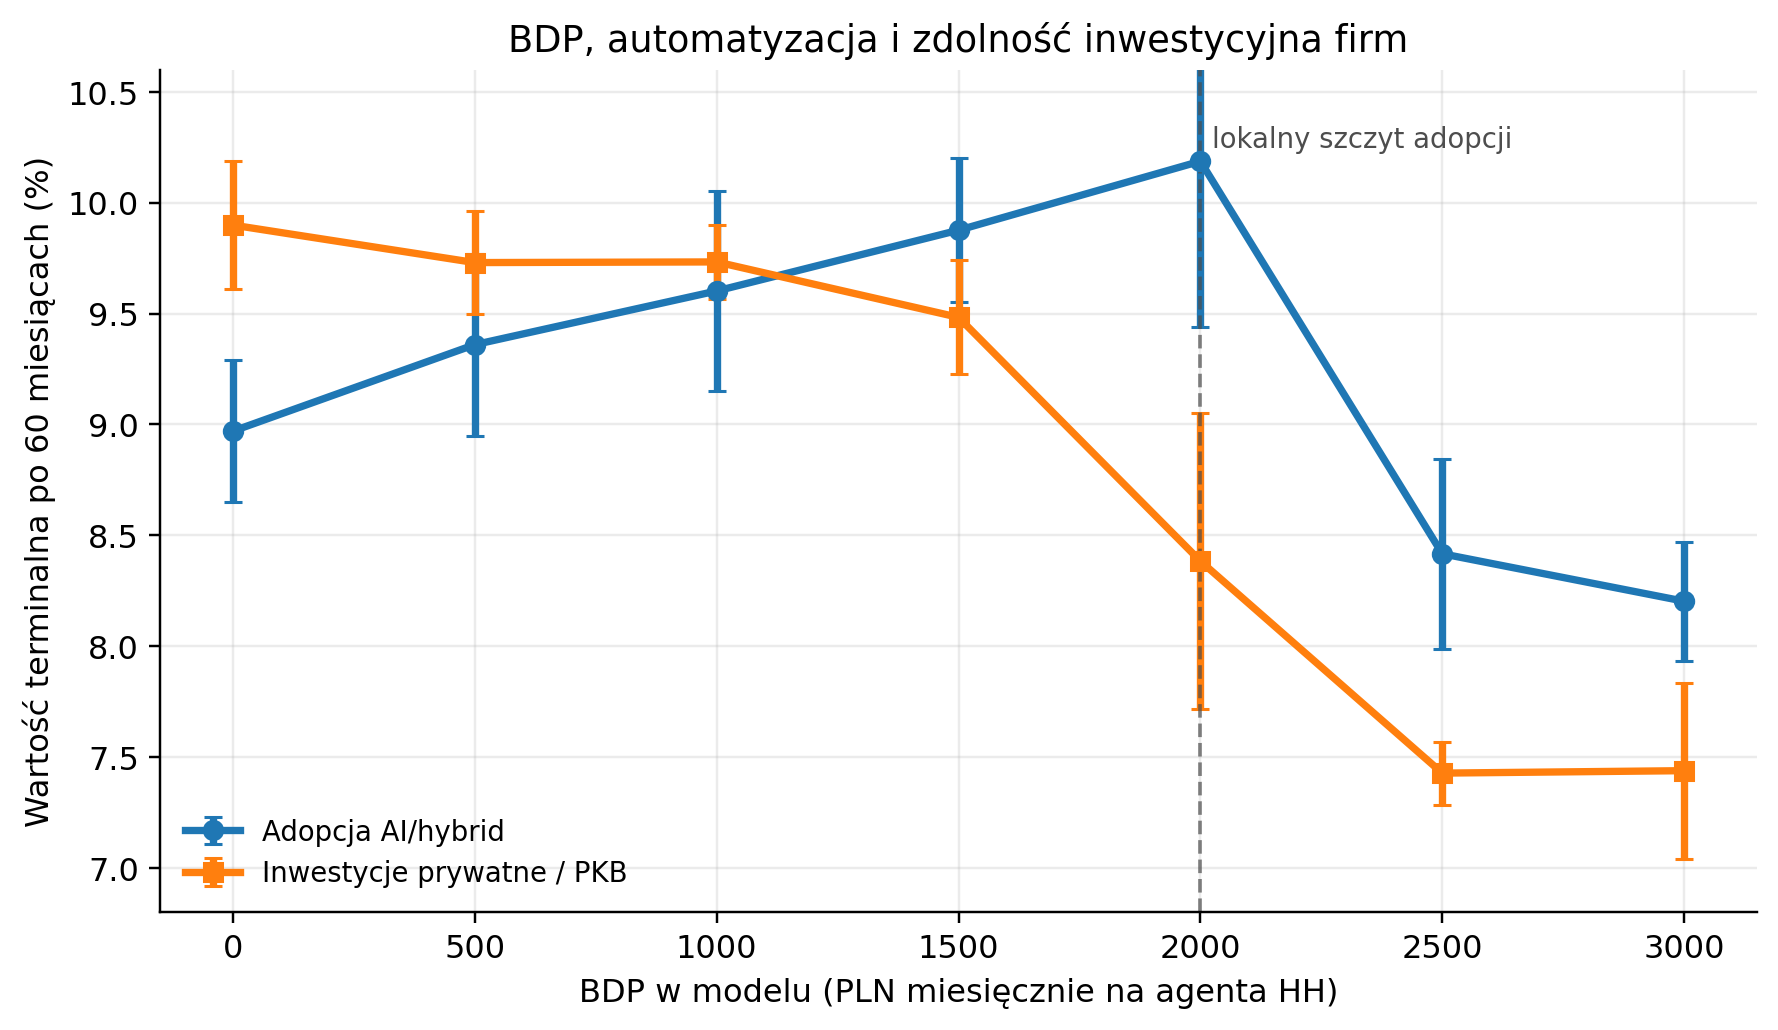
\includegraphics[width=\textwidth]{figures/fig01_bdp_adoption_investment.png}
  \caption{BDP, adopcja AI/hybrid i inwestycje prywatne. Punkty pokazują średnie terminalne dla 10 ziaren losowania, a pionowe odcinki pokazują odchylenie standardowe między ziarnami.}
  \label{fig:bdp-adoption-investment}
\end{figure}

\subsection{Odporność parametru lambda}

Analiza odporności pokazuje, że wynik nie jest czysto mechanicznym skutkiem samego transferu. Przy \(\lambda = 0\), czyli przy braku przełożenia BDP na płacę rezerwową, adopcja AI/hybrid pozostaje blisko wariantu bez BDP i nie tworzy wyraźnej krzywej akceleracji. Przy \(\lambda = 0{,}25\) adopcja rośnie łagodnie wraz z BDP, ale nie pojawia się gwałtowny próg. Oznacza to, że sam kanał popytowo-fiskalny nie wystarcza do mocnej wersji hipotezy.

Najwięcej mówi wariant centralny \(\lambda = 0{,}5\). Pokazuje on zakres umiarkowanego przyspieszenia adopcji: adopcja rośnie z 8,97\% w wariancie bez BDP do 10,19\% przy BDP 2000~PLN, a następnie spada do 8,42\% przy BDP 2500~PLN i 8,20\% przy BDP 3000~PLN. Warianty \(\lambda = 0{,}75\) i \(\lambda = 1\) przesuwają próg w lewo: lokalny szczyt pojawia się już przy BDP 1000~PLN, a wyższe poziomy transferu obniżają inwestycje prywatne i adopcję.

Wniosek z analizy odporności jest jednoznaczny: BDP może być katalizatorem automatyzacji tylko w przedziale pośrednim. Próg absorpcji wymaga jednoczesnej obecności presji płacowo-rezerwowej i kanału fiskalno-finansowego. Przy \(\lambda = 0\) rośnie deficyt i dług, ale adopcja AI/hybrid pozostaje blisko wariantu bez BDP; sam kanał fiskalny nie tworzy więc odwróconego U. Jeśli transfer wpływa na płacę rezerwową zbyt mocno, kanał kosztu pracy, inwestycji i finansowania zaczyna dławić zdolność firm do ucieczki technologicznej. Hipoteza ma więc charakter warunkowy, a nie monotoniczny.

\begin{figure}[H]
  \centering
  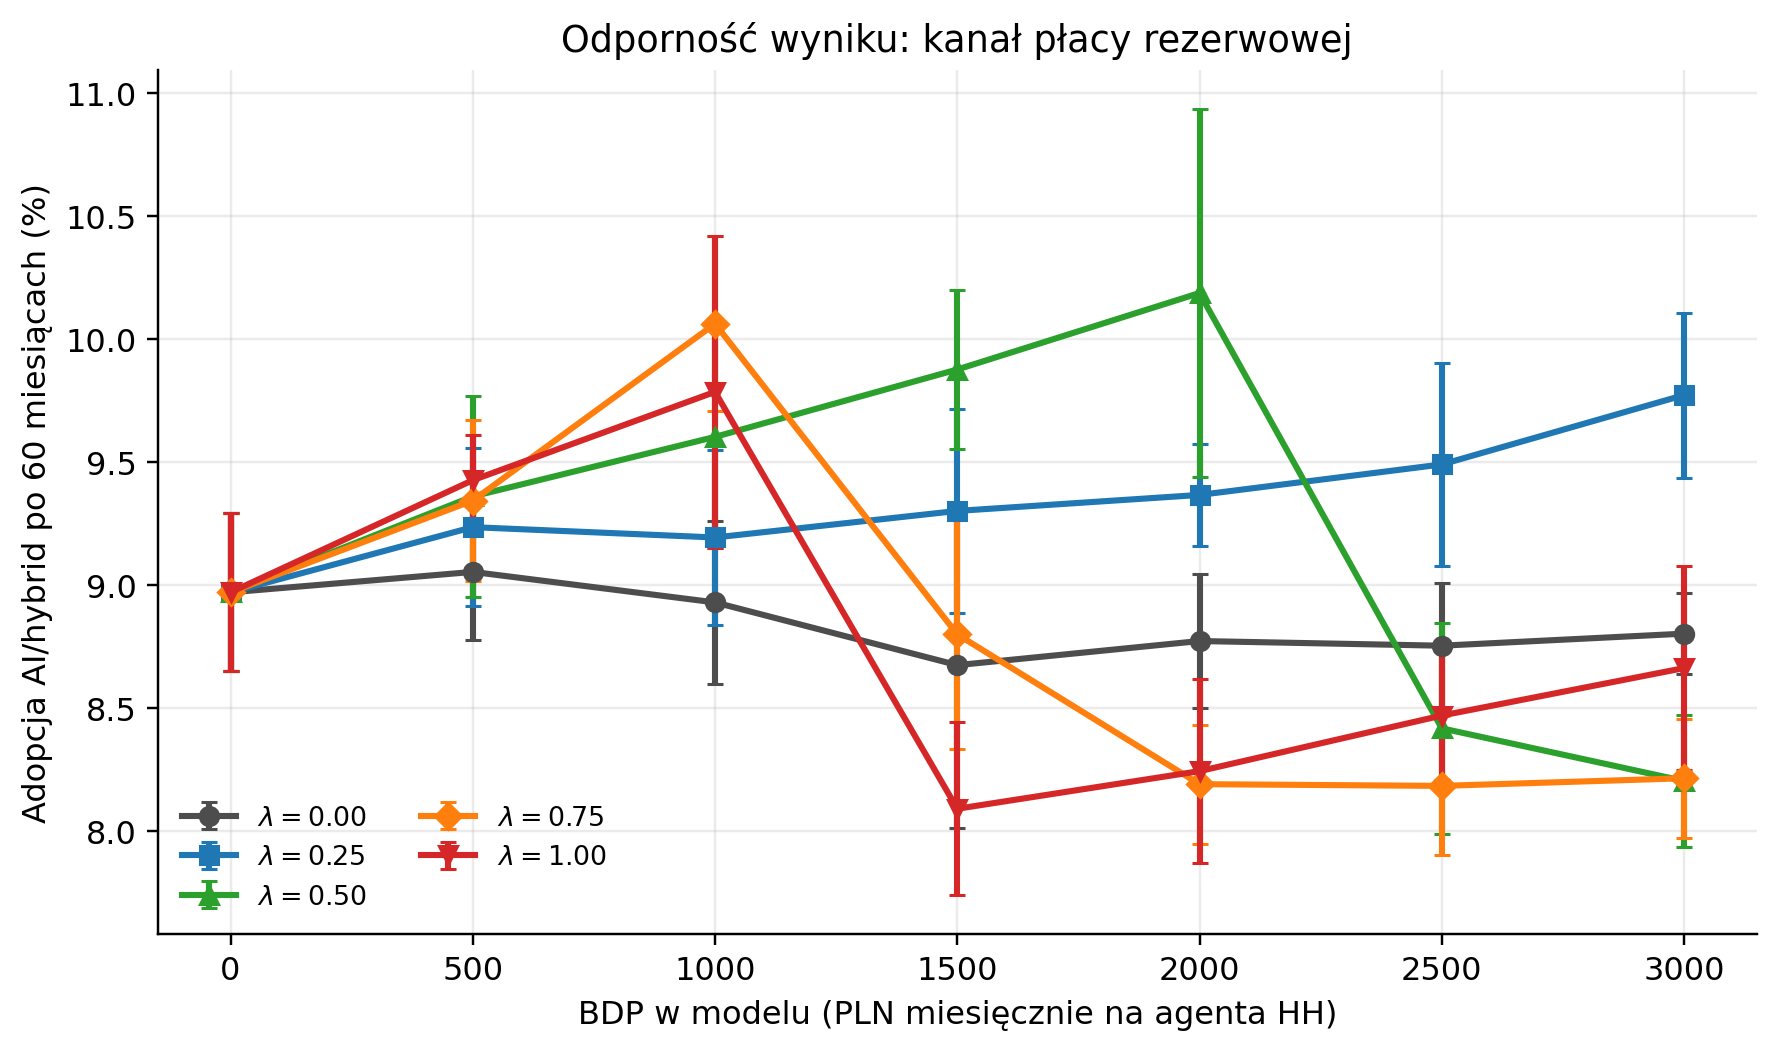
\includegraphics[width=\textwidth]{figures/fig05_lambda_robustness.png}
  \caption{Analiza odporności kanału płacy rezerwowej. Linie pokazują średnią terminalną adopcję AI/hybrid dla 10 ziaren losowania i pięciu wartości \(\lambda\).}
  \label{fig:lambda-robustness}
\end{figure}

\subsection{Ścieżka przejścia sektora firm}

Rysunek~\ref{fig:firm-transition-panel} pokazuje, co kryje się za wynikiem terminalnym. W wariancie BDP 2000~PLN adopcja AI/hybrid rośnie silniej niż w ścieżce bez BDP, ale dzieje się to przy wyraźnie słabszej ścieżce inwestycji prywatnych/PKB. Wysoki wariant BDP 3000~PLN pokazuje, że większa liczba firm nie oznacza automatycznie większej automatyzacji. Liczba aktywnych firm rośnie, ale inwestycje prywatne/PKB pozostają nisko, a adopcja AI/hybrid jest słabsza niż przy BDP 2000~PLN.

Nie jest to wyłącznie efekt wyższego mianownika PKB. W danych terminalnych spada także nominalny strumień prywatnych inwestycji brutto: z około 44,3 mld PLN miesięcznie w wariancie bez BDP do około 37,5 mld PLN przy BDP 2000~PLN i 33,9 mld PLN przy BDP 3000~PLN. W modelu inwestycja firmy jest ograniczana gotówką oraz możliwością pozyskania finansowania zewnętrznego. Wysoki BDP zwiększa deficyt i dług publiczny, podnosi rentowności obligacji publicznych oraz koszt długu korporacyjnego, a równocześnie przez kanał płacy rezerwowej i kursu walutowego pogarsza część kosztów firm. Presja automatyzacyjna rośnie, ale firmy mają mniej przestrzeni bilansowej, aby tę reakcję sfinansować. Ograniczeniem nie jest więc sama liczba podmiotów gospodarczych, lecz zdolność firm do finansowania inwestycji technologicznych.

\begin{figure}[H]
  \centering
  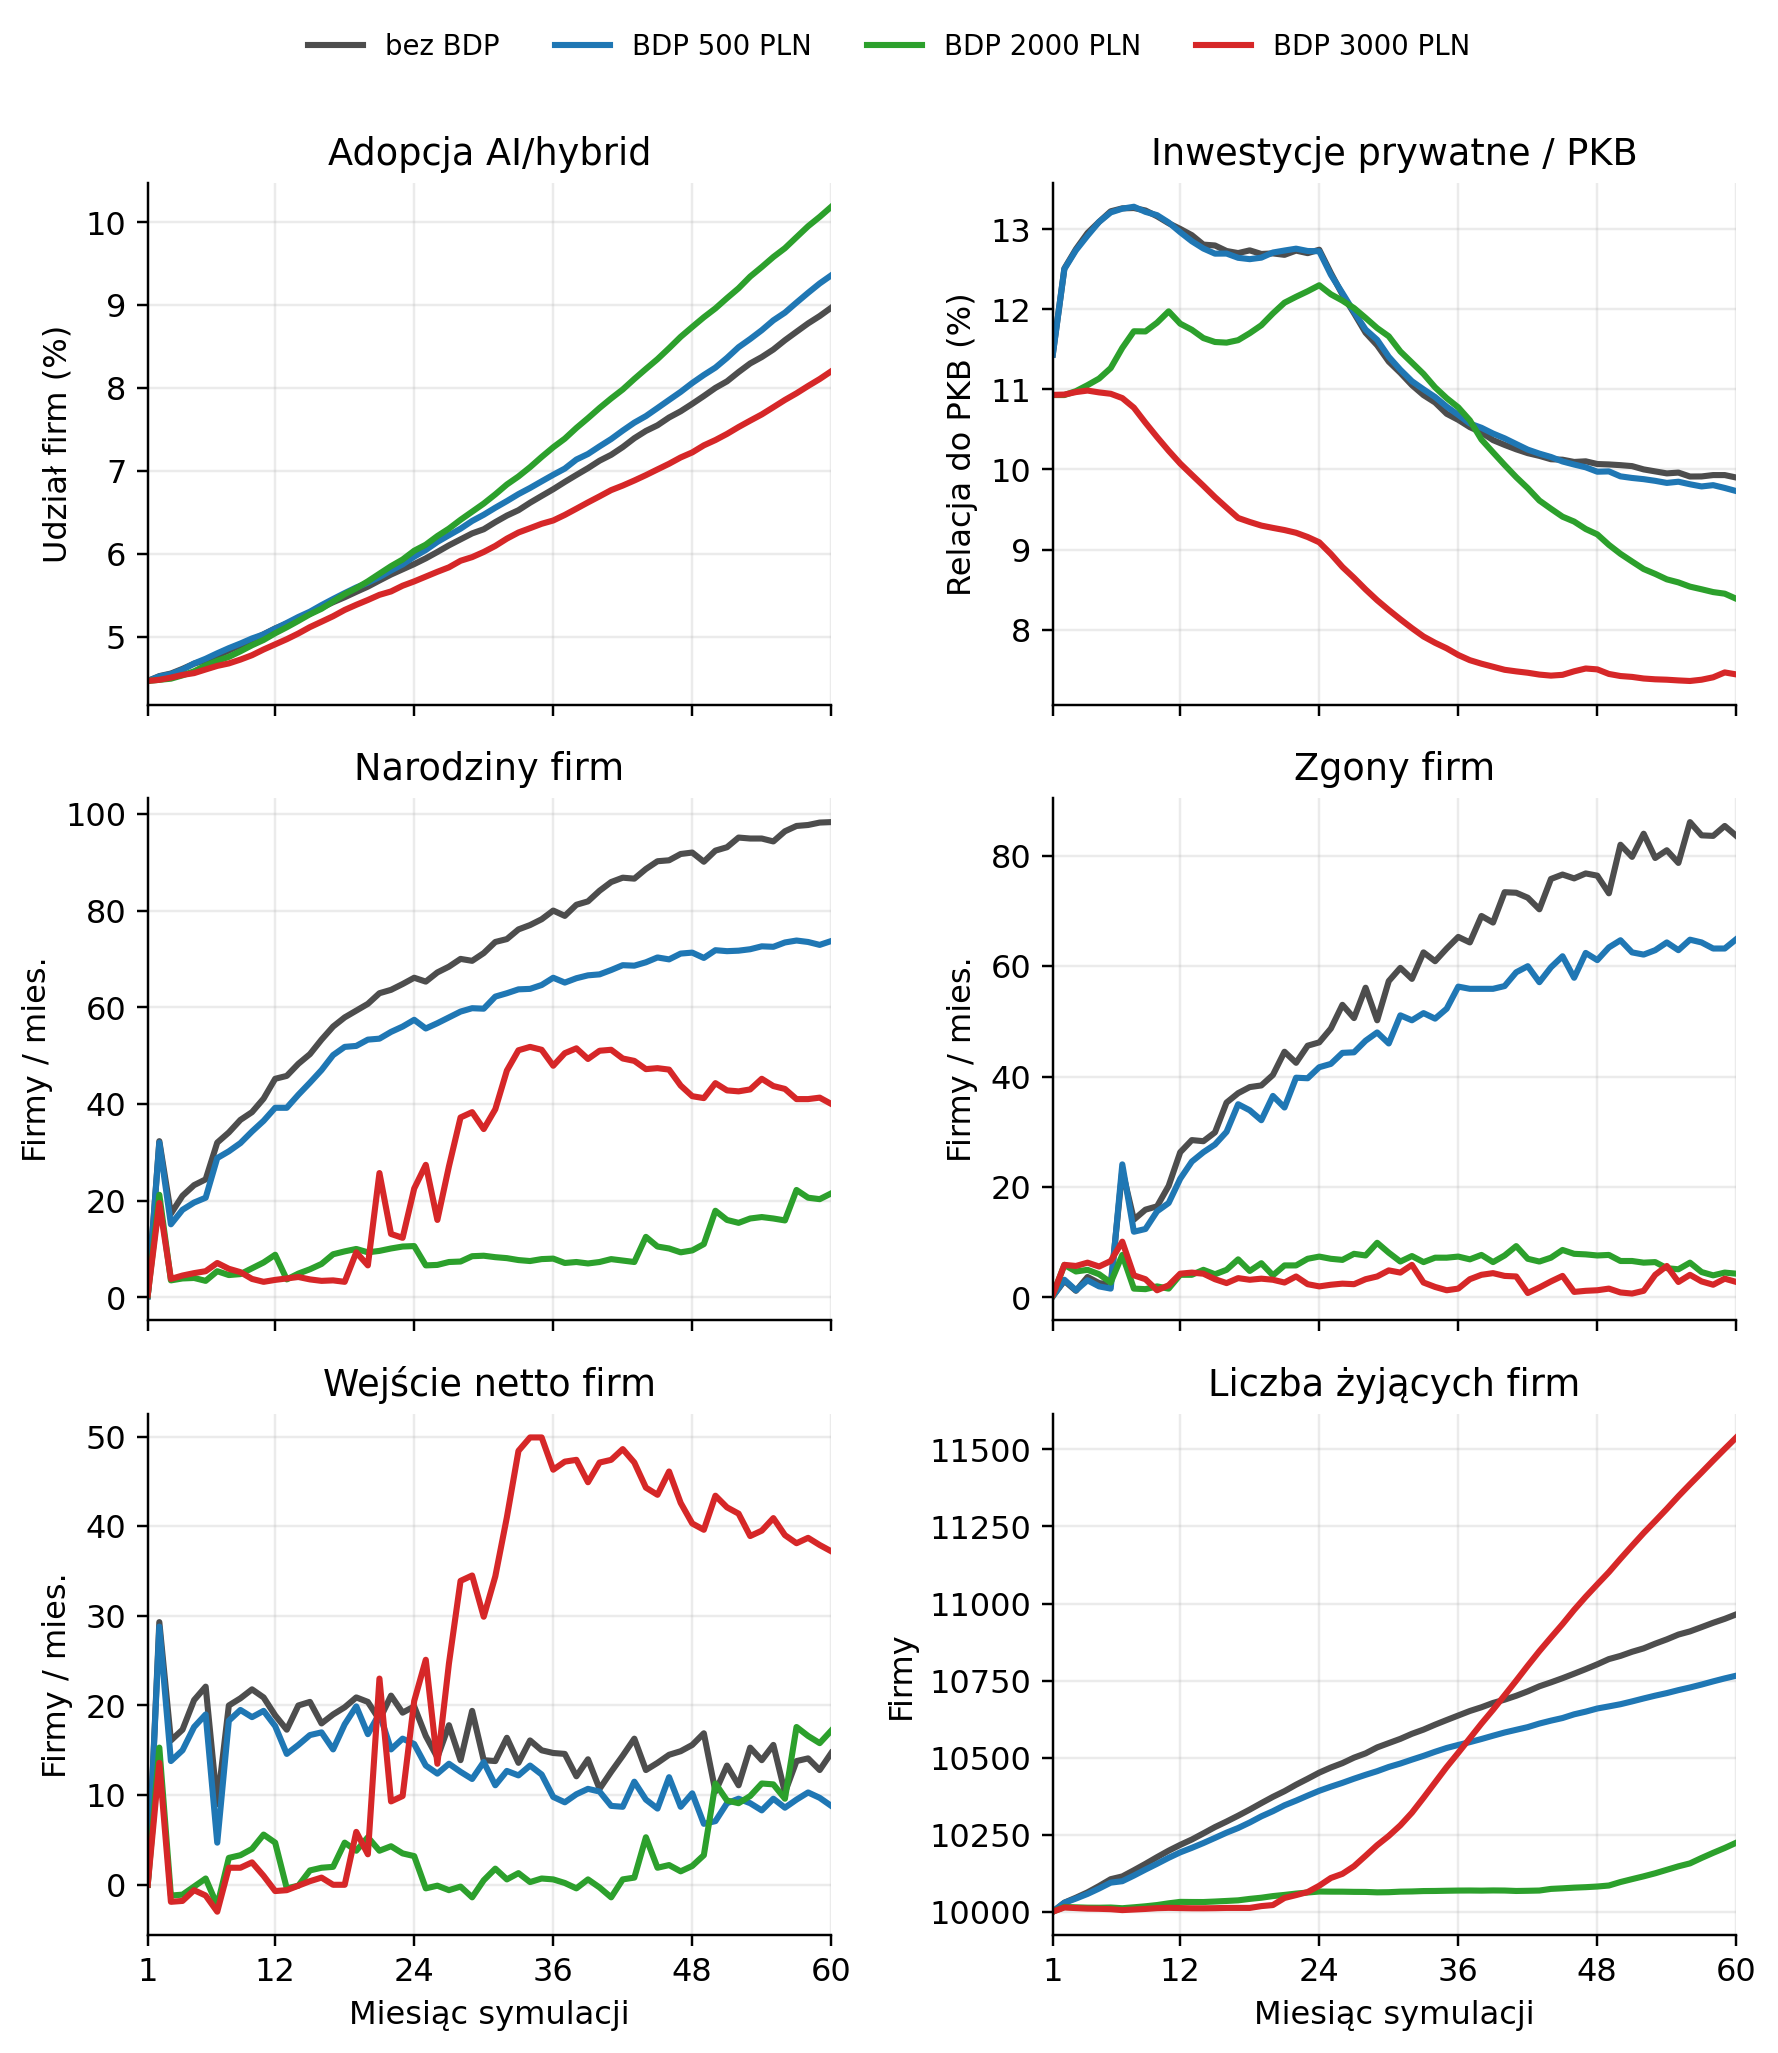
\includegraphics[width=\textwidth]{figures/fig06_firm_transition_panel.png}
  \caption{Ścieżki miesięczne sektora firm dla wybranych poziomów BDP. Linie pokazują średnie z 10 ziaren losowania: wariant bez BDP, dolną kotwicę BDP 500~PLN, wariant lokalnego szczytu adopcji BDP 2000~PLN oraz wysoki impuls BDP 3000~PLN.}
  \label{fig:firm-transition-panel}
\end{figure}

\begin{table}[H]
\centering
\scriptsize
\caption{Demografia firm i struktura wielkości w wariancie centralnym \(\lambda = 0{,}5\), miesiąc 60}
\label{tab:firm-demography-size}
\begin{tabular}{@{}r r r r r r r r@{}}
\toprule
\textbf{BDP} & \textbf{Aktywne} & \textbf{Nowe/mies.} & \textbf{Zamkn./mies.} & \textbf{Mikro \%} & \textbf{Małe \%} & \textbf{Średnie \%} & \textbf{Duże \%} \\
\midrule
0 & 10 965 & 98,3 & 83,6 & 90,87 & 8,23 & 0,71 & 0,19 \\
500 & 10 766 & 73,7 & 64,9 & 90,46 & 8,61 & 0,72 & 0,22 \\
1000 & 10 595 & 53,9 & 46,0 & 89,92 & 9,13 & 0,73 & 0,22 \\
1500 & 10 339 & 26,8 & 23,7 & 88,62 & 10,37 & 0,78 & 0,22 \\
2000 & 10 224 & 21,5 & 4,3 & 88,03 & 10,88 & 0,83 & 0,25 \\
2500 & 11 280 & 40,1 & 2,5 & 94,41 & 4,70 & 0,69 & 0,19 \\
3000 & 11 539 & 40,0 & 2,8 & 96,56 & 2,66 & 0,61 & 0,18 \\
\bottomrule
\end{tabular}
\end{table}


Dane o demografii firm uzupełniają ten wynik. Nie wskazują one na gwałtowną konsolidację rynku przez większe podmioty. W wariancie centralnym \(\lambda = 0{,}5\) pojawia się raczej nieliniowa zmiana struktury firm. Do poziomu BDP 2000~PLN spada zarówno liczba nowych firm, jak i liczba firm kończących działalność: z 98,3 nowych firm i 83,6 firm kończących działalność miesięcznie w wariancie bez BDP do 21,5 nowych firm i 4,3 firm kończących działalność miesięcznie. Jednocześnie udział mikrofirm spada z 90,87\% do 88,03\%, a udział firm małych rośnie z 8,23\% do 10,88\%. Można to interpretować jako zamrożenie selekcji rynkowej połączone z przejściem części firm poza mikrosegment.

Powyżej BDP 2500~PLN wzorzec się odwraca. Liczba firm rośnie do około 11,5 tys., ale wzrost ten odbywa się niemal wyłącznie w segmencie mikrofirm: ich udział wynosi 94,41\% przy BDP 2500~PLN i 96,56\% przy BDP 3000~PLN. Udział firm małych spada natomiast do 2,66\%. To nie jest obraz przejęcia rynku przez większych graczy. Bardziej prawdopodobna interpretacja to bariera skalowania i technologicznego dojrzewania sektora: nowe podmioty mogą powstawać jako mikrofirmy, ale przy wysokim koszcie kapitału i niższej inwestycji prywatnej trudniej im przejść do większych klas wielkości oraz sfinansować automatyzację.

\subsection{Płaca rezerwowa}

Kanał płacy rezerwowej jest aktywny mechanicznie: przy \(\lambda = 0{,}5\) scenariusz BDP 2000~PLN podnosi płacę rezerwową o 1000 PLN. Nie przekłada się to jednak natychmiast na silny wzrost płacy rynkowej. Modelowa płaca rynkowa pozostaje blisko wariantu bez BDP do poziomu BDP 1500~PLN, a wyraźniej rośnie dopiero przy BDP 2500~PLN i BDP 3000~PLN. Sam kanał płacy rezerwowej nie tłumaczy więc wzrostu adopcji AI/hybrid do BDP 2000~PLN.

\subsection{Popyt}

Transfer zwiększa dochód gospodarstw domowych, ale mediana konsumpcji i PKB reagują słabiej. Przy BDP 2000~PLN średni dochód gospodarstw rośnie względem wariantu bez BDP o około 2,1 tys. PLN, natomiast mediana konsumpcji tylko o około 190 PLN. Część impulsu trafia zatem do oszczędności, importu i bilansów, a nie wyłącznie do krajowego popytu finalnego.

\subsection{Panel kontrolny gospodarstw domowych}

Rysunek~\ref{fig:hh-control-panel} pełni funkcję kontroli alternatywnego wyjaśnienia. Gdyby nieliniowość adopcji AI/hybrid wynikała głównie z załamania sytuacji gospodarstw domowych, należałoby oczekiwać wyraźnej zmiany ubóstwa, nierówności albo niewypłacalności gospodarstw. W obecnym eksperymencie takiego sygnału nie widać. Średni dochód gospodarstw i mediana oszczędności rosną wraz z BDP, mediana konsumpcji rośnie umiarkowanie, a wskaźniki dystrybucyjne pozostają stabilne. Gini dochodowy pozostaje w przedziale około 0,28--0,29, stopa ubóstwa relatywnego 50\% mediany pozostaje blisko 13,5--14,3\%, a raportowana metryka bankructw gospodarstw domowych pozostaje zerowa w wariancie centralnym. Ten ostatni wskaźnik traktuję pomocniczo: model nie odtwarza administracyjnej procedury upadłości konsumenckiej, lecz służy do analizy kanałów makro-finansowych.

Ten panel zawęża interpretację wyniku. BDP poprawia płynność gospodarstw domowych, ale nie generuje w horyzoncie 60 miesięcy silnego szoku dystrybucyjnego, który sam tłumaczyłby próg automatyzacji. Nieliniowość adopcji należy więc wiązać przede wszystkim z interakcją kanału firmowego, płacowo-rezerwowego i fiskalno-finansowego: kosztem pracy, kosztem kapitału, inwestycjami prywatnymi oraz zdolnością firm do sfinansowania reakcji technologicznej.

\begin{figure}[H]
  \centering
  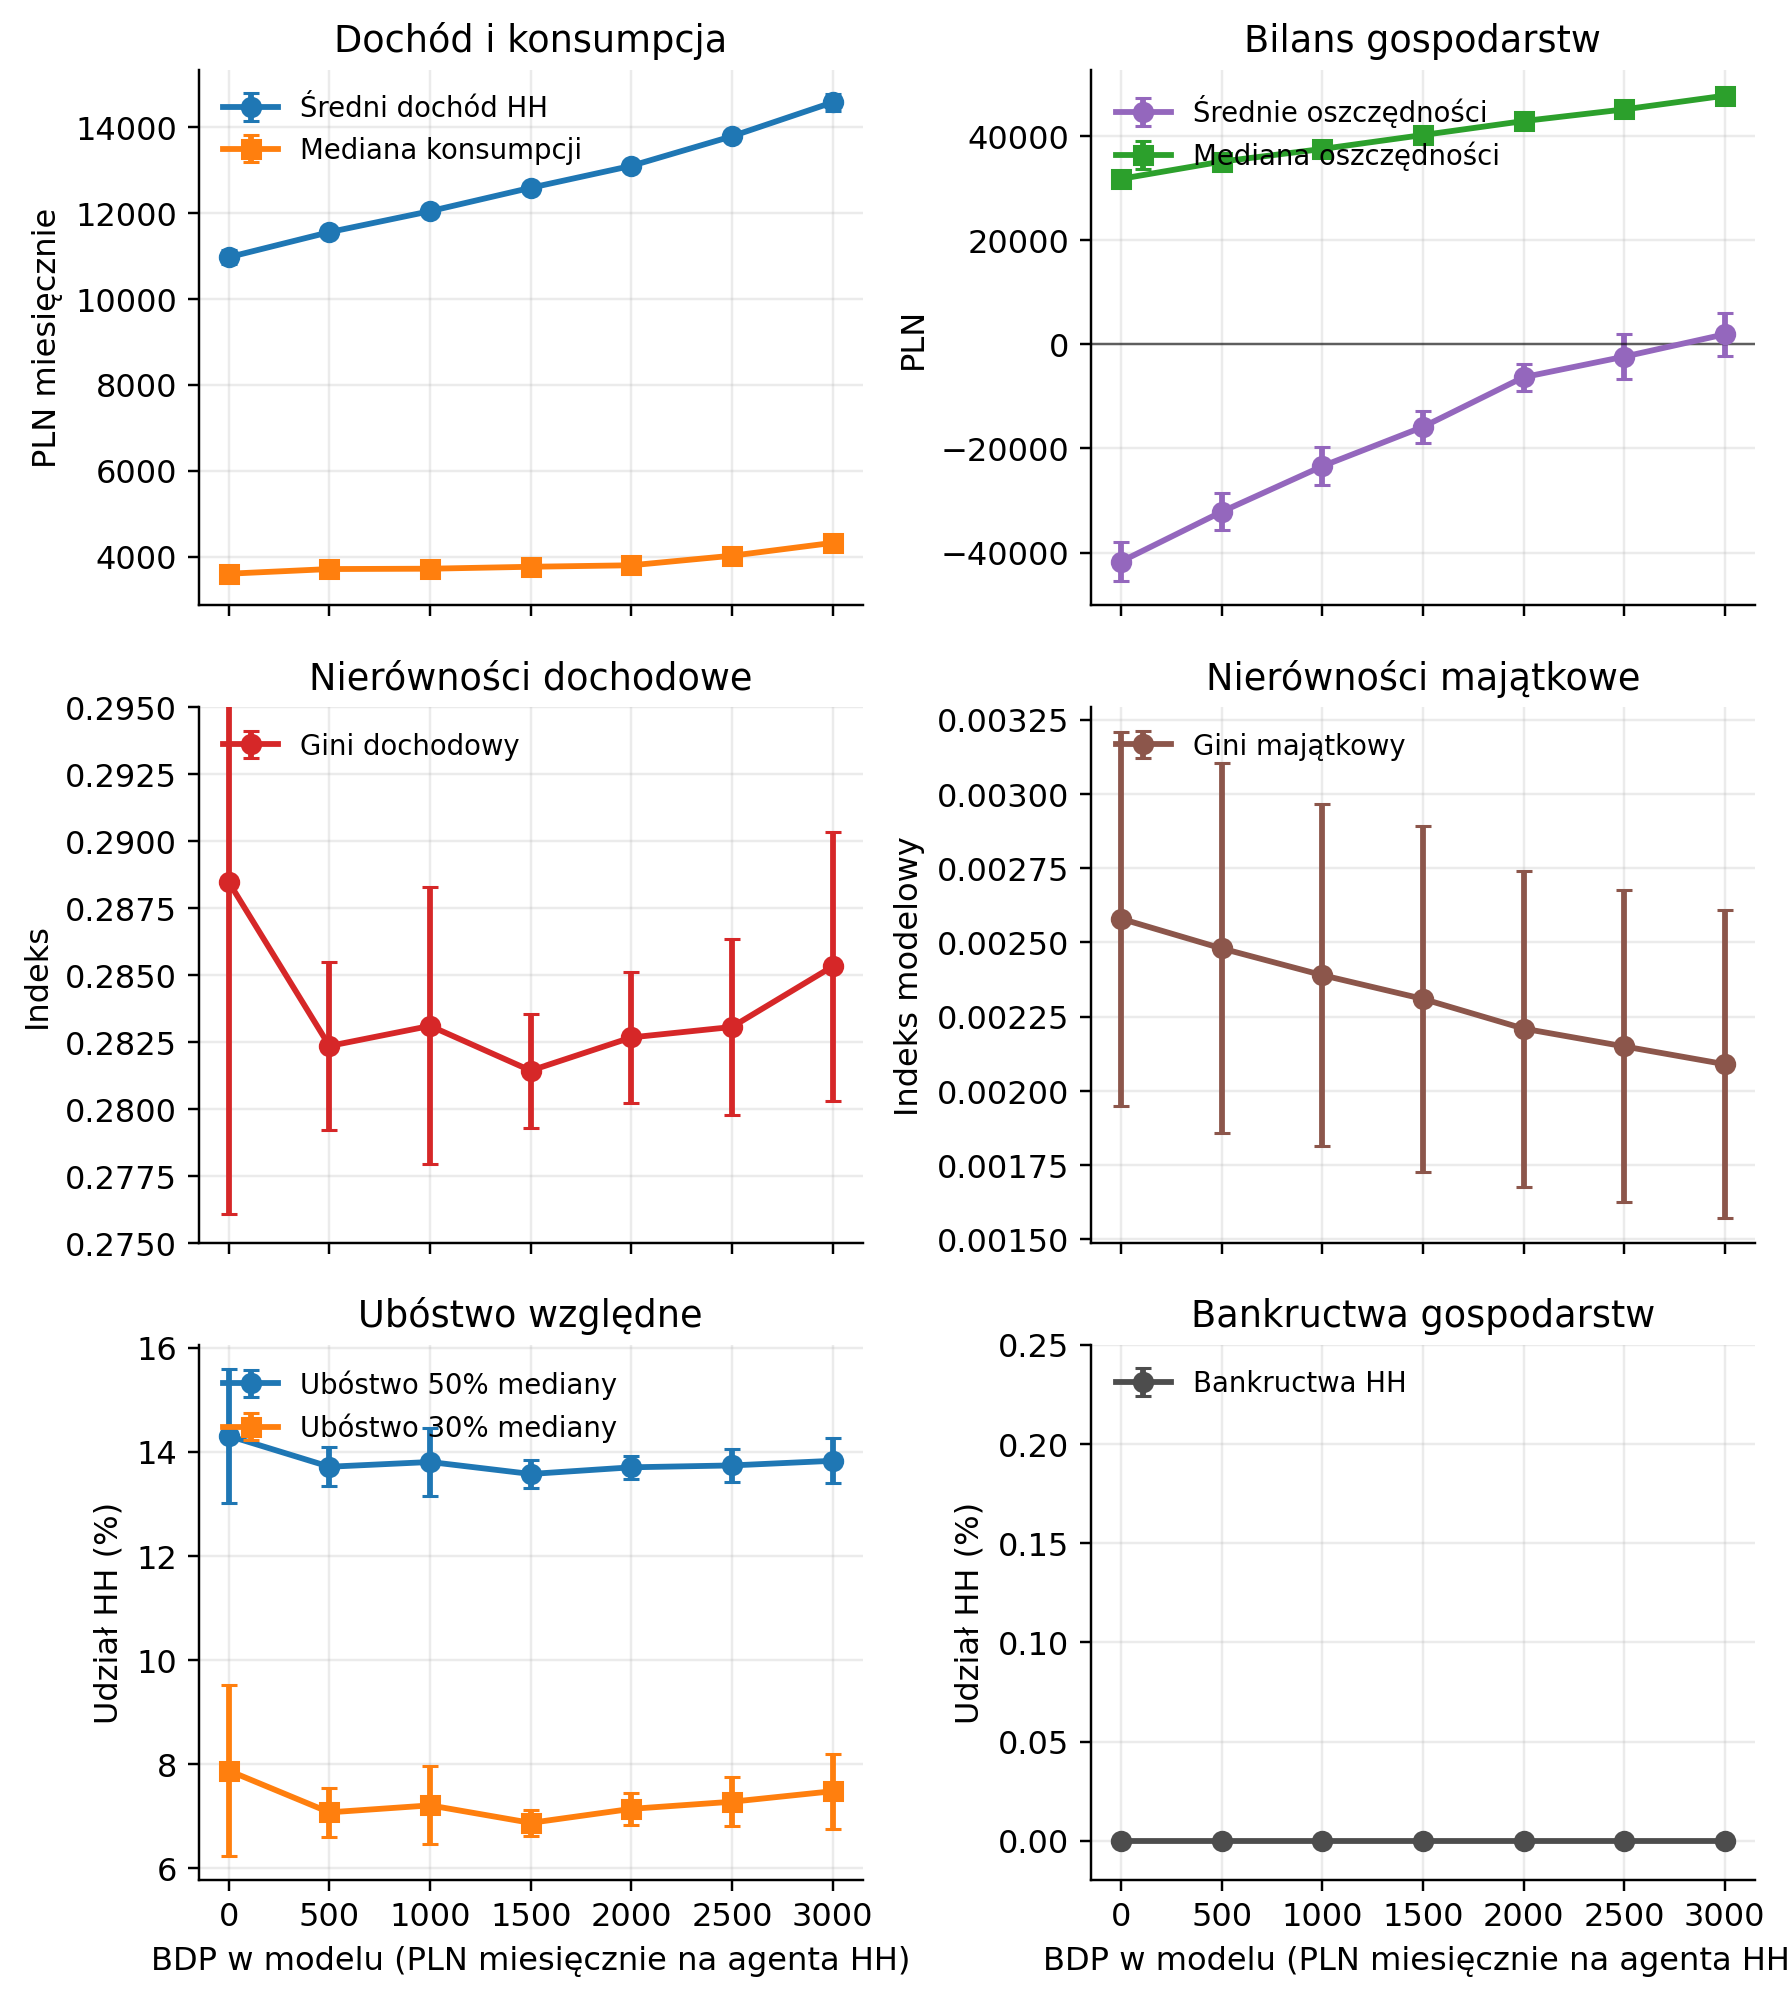
\includegraphics[width=\textwidth]{figures/fig07_hh_control_panel.png}
  \caption{Panel kontrolny gospodarstw domowych. Punkty pokazują średnie terminalne dla 10 ziaren losowania, a pionowe odcinki pokazują odchylenie standardowe między ziarnami.}
  \label{fig:hh-control-panel}
\end{figure}

\subsection{Inflacja i koszt kapitału}

Inflacja i stopa referencyjna NBP rosną umiarkowanie. Silniejszy sygnał pojawia się w koszcie finansowania rynkowego: rentowność obligacji i koszt długu korporacyjnego rosną wraz z poziomem BDP. To przesuwa interpretację z prostego kanału stopy NBP na kanał kosztu kapitału, obejmujący dług publiczny, obligacje korporacyjne i finansowanie inwestycji \parencite{blanchard2019}.

\begin{figure}[H]
  \centering
  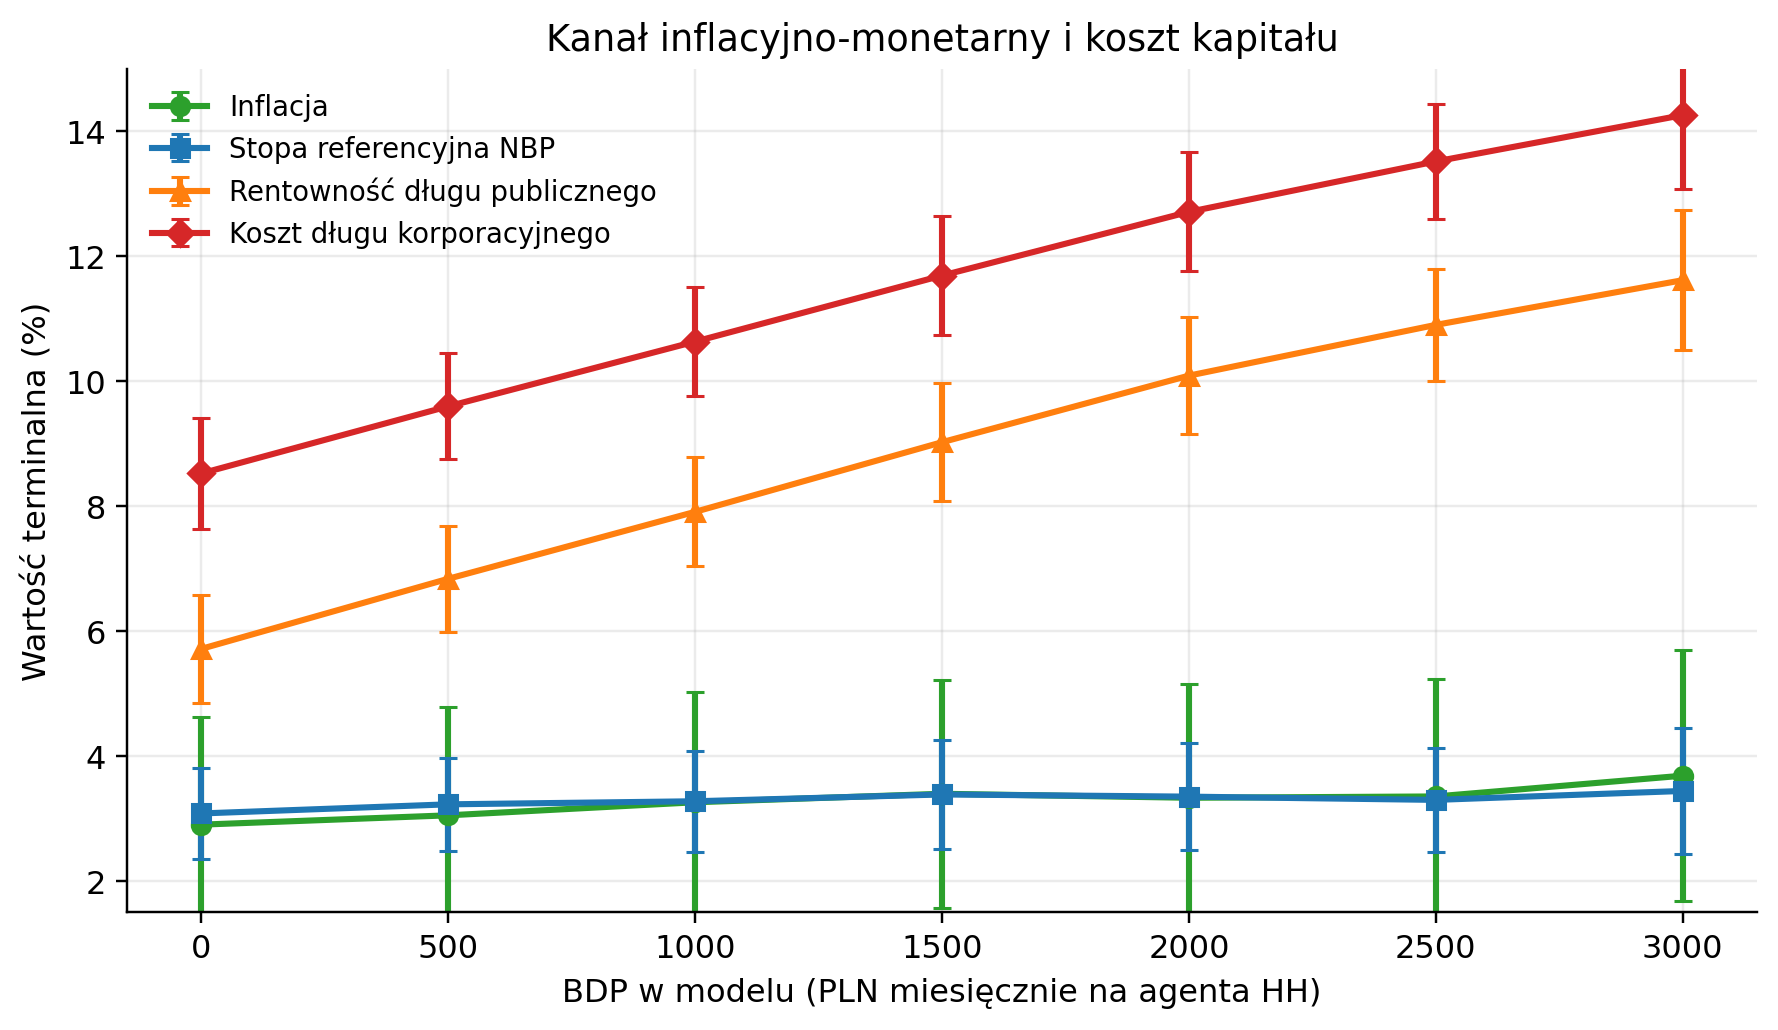
\includegraphics[width=\textwidth]{figures/fig03_bdp_cost_of_capital.png}
  \caption{Kanał inflacyjno-monetarny i koszt kapitału: inflacja, stopa NBP, rentowność długu publicznego i koszt długu korporacyjnego.}
  \label{fig:bdp-cost-capital}
\end{figure}

\subsection{Fiskus i dług}

Kanał fiskalno-dłużny jest najsilniejszy i monotoniczny \parencite{owsiak2017,mf2025debtStrategy,imf2026polandArticleIV}. Dług/PKB rośnie z 69,34\% w wariancie bez BDP do 97,12\% przy BDP 2000~PLN i 106,73\% przy BDP 3000~PLN. Deficyt/PKB rośnie z 7,69\% do odpowiednio 14,20\% i 16,55\%. W ujęciu różnicy względem wariantu bez BDP oznacza to wzrost długu o 27,77 pp PKB przy BDP 2000~PLN i 37,39 pp PKB przy BDP 3000~PLN; deficyt rośnie odpowiednio o 6,51 pp i 8,86 pp PKB. Przy wysokich poziomach transferu kanał fiskalno-dłużny zaczyna dominować nad pozytywnym kanałem popytowym, ale analiza \(\lambda = 0\) pokazuje, że sam wzrost deficytu i długu nie wystarcza do wyjaśnienia spadku adopcji AI/hybrid. Dla tej tezy decyduje interakcja z kanałem płacy rezerwowej i inwestycji firm.

\begin{figure}[H]
  \centering
  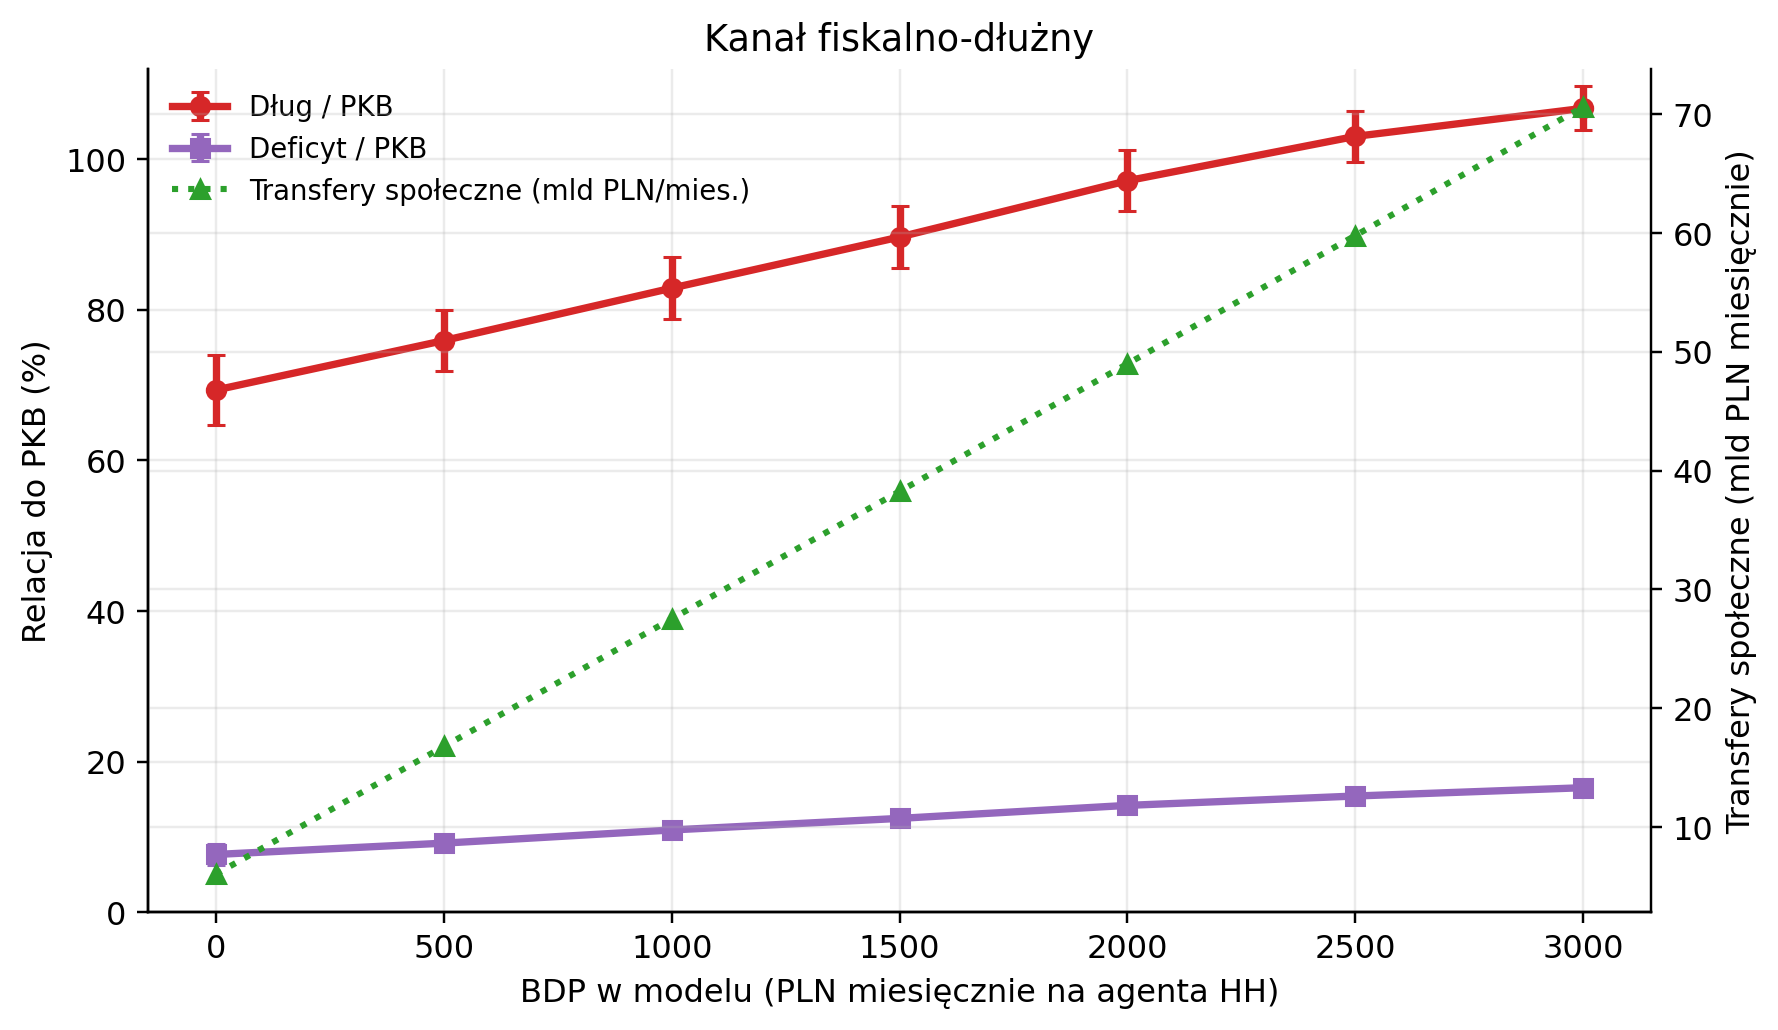
\includegraphics[width=\textwidth]{figures/fig02_bdp_fiscal_stress.png}
  \caption{Kanał fiskalno-dłużny: dług/PKB, deficyt/PKB oraz miesięczne transfery społeczne.}
  \label{fig:bdp-fiscal-stress}
\end{figure}

\subsection{Sektor zewnętrzny}

PLN słabnie, import rośnie, a rachunek bieżący pogarsza się. Przy BDP 3000~PLN kurs PLN/EUR jest o około 3,2\% wyższy niż w wariancie bez BDP, import o około 6,5\% wyższy, a rachunek bieżący pogarsza się o około 3,22 pp PKB względem ścieżki bez BDP. Część impulsu popytowego odpływa więc przez import i kanał kursowy.

\begin{figure}[H]
  \centering
  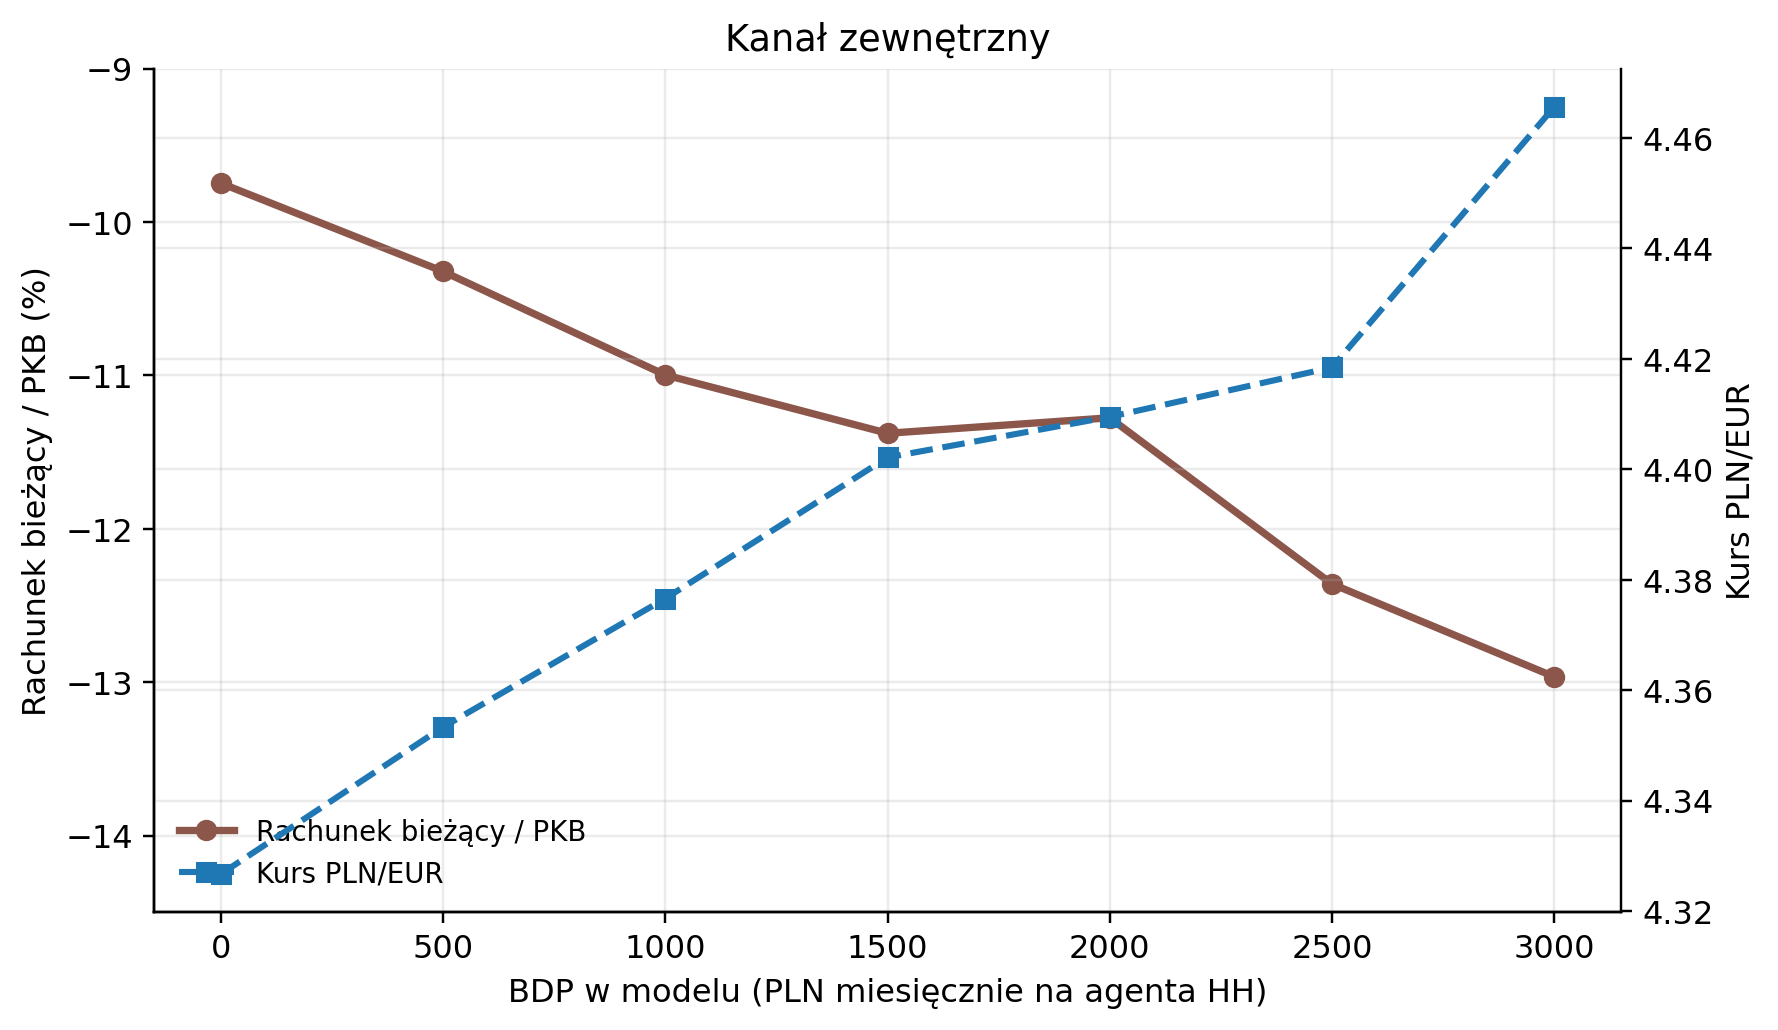
\includegraphics[width=\textwidth]{figures/fig04_bdp_external_channel.png}
  \caption{Kanał zewnętrzny: rachunek bieżący do PKB oraz kurs PLN/EUR.}
  \label{fig:bdp-external-channel}
\end{figure}

\subsection{Kredyt i banki}

W eksperymencie nie widać kryzysu bankowego. Nie występują upadłości banków, wskaźniki CAR/LCR/NSFR pozostają wysokie, a NPL nie rosną monotonicznie. Ograniczenie automatyzacji przy wysokim BDP nie wynika z załamania sektora bankowego, lecz raczej z pogorszenia opłacalności i zdolności finansowania inwestycji prywatnych.

\subsection{Automatyzacja i inwestycje}

Adopcja AI/hybrid rośnie do BDP 2000~PLN, ale równolegle prywatne inwestycje/PKB spadają z 9,90\% w wariancie bez BDP do 8,38\%. Przy BDP 2500~PLN i BDP 3000~PLN inwestycje prywatne/PKB spadają do około 7,4\%, a adopcja AI/hybrid obniża się poniżej wariantu bez BDP. To wskazuje na próg absorpcji w wariancie deficytowym: firmy mogą reagować automatyzacją tylko tak długo, jak mają zdolność finansowania tej reakcji i jednocześnie odczuwają presję po stronie płacy rezerwowej.

Dlatego eksperyment wspiera wersję warunkową hipotezy. Deficytowo finansowany BDP może przyspieszać automatyzację w przedziale, w którym presja kosztowa i popytowa nie ograniczają zdolności inwestycyjnej sektora prywatnego. Po przekroczeniu progu wynikającego z interakcji presji płacowo-rezerwowej oraz ograniczeń fiskalno-finansowych gospodarka nie przechodzi do szybszej automatyzacji, lecz do niższej dynamiki inwestycji prywatnych, pogorszenia bilansu zewnętrznego i silniejszego obciążenia długu publicznego.

\section{Implikacje menedżerskie}

Z perspektywy zarządu najważniejszy wniosek nie brzmi: \textit{BDP wymusza automatyzację}. Brzmi raczej: \textit{BDP zmienia warunki graniczne decyzji inwestycyjnej}. Program transferowy tej skali zmienia jednocześnie płace, popyt, koszt kapitału, kurs walutowy, dostępność kredytu i oczekiwaną rentowność projektów.

Reakcją firmy nie powinno być więc hasło „automatyzować szybciej”. Wynik eksperymentu pokazuje, że umiarkowany BDP może sprzyjać adopcji AI/hybrid, ale przy wysokim transferze presja płacowo-rezerwowa spotyka się z pogorszeniem warunków fiskalno-finansowych. Automatyzacja pozostaje decyzją CapEx: wymaga gotówki, zdolności kredytowej, stabilnego finansowania, kontroli ryzyka kursowego i czasu na wdrożenie.

Granica interpretacji jest ważna. Wprost z modelu wynikają przede wszystkim wnioski o koszcie kapitału, inwestycjach prywatnych, długu, deficycie, kursie i adopcji AI/hybrid. Zalecenia dotyczące portfela projektów, zatrudnienia i FX są menedżerskim przełożeniem tych kanałów, a nie dodatkowymi zmiennymi estymowanymi przez model.

\begin{table}[H]
\centering
\scriptsize
\caption{Macierz decyzji zarządczych po ogłoszeniu scenariusza BDP}
\label{tab:managerial-decision-matrix}
\begin{tabularx}{\textwidth}{@{}>{\raggedright\arraybackslash}p{0.21\textwidth}>{\raggedright\arraybackslash}p{0.25\textwidth}>{\raggedright\arraybackslash}p{0.22\textwidth}>{\raggedright\arraybackslash}X@{}}
\toprule
\textbf{Decyzja zarządcza} & \textbf{Kanał ryzyka} & \textbf{Metryki do monitorowania} & \textbf{Rekomendowana reakcja} \\
\midrule
CapEx teraz czy odroczenie inwestycji &
BDP zwiększa presję automatyzacyjną, ale przy wysokim transferze rośnie koszt kapitału i słabnie ścieżka inwestycji prywatnych. &
Inwestycje prywatne/PKB, koszt długu korporacyjnego, rentowność obligacji, dług/PKB, deficyt/PKB &
Testować projekty w scenariuszach kosztu kapitału. Przy umiarkowanym BDP przyspieszać projekty o krótkim paybacku; przy wysokim BDP chronić płynność i selektywność CapEx. \\
\addlinespace
Automatyzacja selektywna czy pełna &
Presja płacowa nie działa równomiernie na procesy, a finansowanie technologii staje się ograniczeniem. &
Adopcja AI/hybrid, adopcja sektorowa, płaca rynkowa, inwestycje prywatne &
Priorytetyzować procesy pracochłonne, powtarzalne i szybkie we wdrożeniu. Traktować AI jako portfel projektów, nie jako jeden program transformacyjny dla całej firmy. \\
\addlinespace
Struktura zatrudnienia i wynagrodzeń &
BDP może podnosić płacę rezerwową, ale nie musi natychmiast podnosić płacy rynkowej. &
Płaca rynkowa, płaca zatrudnionych, bezrobocie, płaca rezerwowa, konsumpcja HH &
Mapować stanowiska według podatności na automatyzację, wartości relacyjnej i kosztu utraty kompetencji. Łączyć automatyzację z retencją ról krytycznych i reskillingiem. \\
\addlinespace
Finansowanie długiem czy środkami własnymi &
Wysoki BDP zwiększa deficyt i dług publiczny, co może podnosić koszt finansowania rynkowego i ograniczać apetyt banków na ryzyko. &
Koszt długu korporacyjnego, stopa NBP, NPL, CAR, LCR, NSFR, kredyt/PKB &
Przesunąć analizę z samego NPV na odporność finansowania: bufory gotówkowe, linie kredytowe uzgodnione wcześniej, dłuższy tenor i finansowanie etapowe. \\
\addlinespace
Zabezpieczenie kursowe i import technologii &
Automatyzacja często wymaga importowanych maszyn, licencji, komponentów lub usług chmurowych; słabszy PLN podnosi koszt wdrożenia. &
Kurs PLN/EUR, rachunek bieżący/PKB, import, ceny importu, koszt długu walutowego &
Traktować FX jako część uzasadnienia inwestycyjnego. Zabezpieczać ekspozycję walutową, negocjować walutę kontraktów i analizować lokalne alternatywy dostaw. \\
\bottomrule
\end{tabularx}
\end{table}

\subsection{Priorytety decyzji}

Pierwszy priorytet to dyscyplina CapEx. Firma nie powinna pytać wyłącznie, czy projekt obniży koszt jednostkowy pracy. Powinna pytać, czy zachowuje dodatnią wartość przy wyższym koszcie długu, słabszym PLN, droższej technologii importowanej i słabszej dostępności finansowania. W przedziale umiarkowanego BDP racjonalne może być przyspieszenie projektów o krótkim czasie zwrotu. Przy wysokim BDP większą wartość ma ochrona bilansu: mniej projektów, mniejszy jednorazowy CapEx, większy udział projektów modułowych i większy bufor gotówkowy.

Praktycznie oznacza to zmianę kryterium kwalifikacji projektów. Projekt automatyzacyjny powinien przejść osobno test zwrotu operacyjnego, test finansowania i test ryzyka wdrożenia. Inwestycja atrakcyjna przy stabilnym WACC może przestać być akceptowalna, jeśli wymaga długu refinansowanego w okresie wzrostu rentowności albo dużych płatności walutowych.

Drugi priorytet to automatyzacja selektywna. Wynik modelu nie wspiera strategii „automatyzować wszystko”. Jeżeli koszt kapitału rośnie razem z kosztem pracy, wygrywają projekty o dużej powtarzalności, wysokim udziale pracy w koszcie, niskiej niepewności popytu i szybkim efekcie na marży. Rola zarządu przesuwa się z pytania „czy wdrożyć AI” na pytanie „gdzie AI ma największą odporność bilansową”.

To sprzyja mniejszym projektom o krótkim czasie zwrotu: automatyzacji back-office, kontroli jakości, planowania zapasów, obsługi wyjątków albo predykcyjnego utrzymania ruchu. Duże programy transformacyjne pozostają możliwe, ale wymagają etapowania i punktów decyzyjnych, w których zarząd może zatrzymać projekt bez utraty całości nakładów.

Trzeci priorytet to zarządzanie zatrudnieniem bez reakcji panicznej. Kanał płacy rezerwowej jest aktywny, ale w modelu płaca rynkowa reaguje wyraźniej dopiero przy wyższych poziomach BDP. Firma powinna więc rozdzielić role rutynowe, relacyjne i krytyczne operacyjnie. Odpowiedzią nie musi być prosta redukcja etatów; może nią być zmiana struktury pracy: mniej czynności rutynowych, więcej nadzoru nad procesami, obsługi wyjątków, utrzymania automatyzacji i reskillingu.

Czwarty priorytet to finansowanie i FX. Wysoki BDP nie musi wywołać natychmiastowego kryzysu bankowego, aby ograniczyć inwestycje. Wystarczy, że rosną koszt długu, wymogi zabezpieczeń, ryzyko refinansowania i koszt importowanej technologii. Dlatego ekspozycja walutowa powinna wejść do uzasadnienia inwestycyjnego od pierwszego dnia: waluta kontraktu, harmonogram płatności, udział komponentów importowanych, serwis, licencje i ryzyko długu walutowego.

Najbardziej podatne są firmy o niskiej marży, wysokiej dźwigni i dużym udziale importowanych komponentów technologicznych. Dla nich BDP może jednocześnie zwiększyć presję kosztu pracy i podnieść cenę kapitału. Jeżeli bilans nie ma bufora, bodziec do automatyzacji nie zamienia się w inwestycję, tylko w presję na marżę.

\subsection{Konkluzja dla zarządu}

BDP należy traktować jako szok strategiczny dla bilansu firmy. Nie jest to wyłącznie program społeczny ani prosty impuls popytowy. Jest to zmiana układu cen względnych i warunków finansowania: pracy, kapitału, długu, waluty, importu i ryzyka fiskalnego.

Najlepsza reakcja zarządu nie polega na maksymalizacji tempa automatyzacji, lecz na utrzymaniu zdolności do sfinansowania właściwych projektów w odpowiednim momencie. W przedziale umiarkowanego BDP przewagę może dać szybka, selektywna automatyzacja procesów o wysokim zwrocie. W przedziale wysokiego BDP przewagę może dać odporność bilansu: płynność, kontrola dźwigni, zabezpieczenie kursowe i dyscyplina CapEx.

Praktyczna kolejność decyzji jest więc następująca. Najpierw trzeba ustalić, które procesy naprawdę tworzą ekspozycję na presję płacową. Następnie sprawdzić, czy projekt automatyzacji ma finansowanie odporne na wyższy koszt długu i słabszy PLN. Dopiero na końcu warto rozstrzygać skalę wdrożenia technologii. W scenariuszu BDP przewagę ma nie firma, która najszybciej ogłasza automatyzację, lecz firma, która najdłużej zachowuje zdolność finansowania dobrych projektów.

\section{Ograniczenia, falsyfikacja i dalsza praca}

Wynik tej pracy należy czytać jako kontrfaktyczny eksperyment obliczeniowy, a nie punktową prognozę makroekonomiczną dla Polski. \amor{} bada ścieżki alternatywne względem wariantu bez BDP i pokazuje mechanizm: przy deficytowym finansowaniu transfer może zwiększać presję automatyzacyjną tylko do momentu, w którym kanał płacowo-rezerwowy i fiskalno-finansowy zaczynają ograniczać zdolność firm do finansowania inwestycji. Dlatego centralna interpretacja opiera się na różnicach względem ścieżki bez BDP, nie na absolutnych poziomach terminalnych.

\subsection{Diagnostyka wariantu bez BDP}

Model startuje ze skalibrowanego punktu Polski 2026-04-30, ale wartości z pierwszego miesiąca obejmują już przepływy i księgowania wykonane przez model. Zewnętrzne punkty odniesienia pochodzą z raportu inflacyjnego NBP, uchwały RPP z 4 marca 2026 r., tablic GUS, strategii długu Ministerstwa Finansów oraz Article IV MFW dla Polski \parencite{nbp2026inflationReport,nbp2026rppResolution,gus2026unemploymentMarch,gus2026gdp2025Preliminary,mf2025debtStrategy,imf2026polandArticleIV}.

\begin{table}[H]
\centering
\scriptsize
\caption{Diagnostyka wariantu bez BDP: punkt odniesienia zewnętrzny, pierwszy wynik miesięczny i ścieżka po 60 miesiącach}
\label{tab:baseline-plausibility}
\begin{tabularx}{\textwidth}{@{}L{0.20\textwidth}L{0.20\textwidth}rrX@{}}
\toprule
Zmienna & Punkt odniesienia zewnętrzny & Model, m1 & Bez BDP, m60 & Interpretacja \\
\midrule
Inflacja CPI & 3,0\% w III 2026 / projekcja blisko celu & 3,33\% & 2,90\% & wejście i koniec ścieżki pozostają blisko celu inflacyjnego \\
Stopa referencyjna NBP & 3,75\% od 05.03.2026 & 3,55\% & 3,08\% & m1 odzwierciedla regułę reakcji modelu, nie literalny punkt decyzji RPP \\
Bezrobocie & 6,1\% rejestrowane, koniec III 2026 & 6,09\% & 7,40\% & start bliski kotwicy; wariant bez BDP generuje pogorszenie rynku pracy \\
Dług publiczny/PKB & ok. 53--66\%, zależnie od definicji PDP/EDP & 47,09\% & 69,34\% & ścieżka bez BDP generuje wzrost długu; poziom terminalny nie jest prognozą punktową \\
Deficyt/PKB & ok. 6--7\% w prognozach 2025--2026 & 13,59\% & 7,69\% & m1 obejmuje startowe przepływy wykonania modelu; porównania BDP opierają się na różnicach względem wariantu bez BDP \\
Rachunek bieżący/PKB & około -1\% PKB w projekcji MFW 2026 & -5,23\% & -9,75\% & poziom bezwzględny nie jest prognozą; interpretowane są zmiany względem tej samej ścieżki bez BDP \\
Inwestycje prywatne/PKB & GUS: stopa inwestycji ogółem 17,0\% PKB w 2025; prywatny odpowiednik jest węższy & 11,44\% & 9,90\% & zmienna modelowa jest węższa od GFCF ogółem; używana głównie jako kontrfaktyczna delta \\
\bottomrule
\end{tabularx}
\end{table}


Tabela~\ref{tab:baseline-plausibility} pokazuje, że wariant bez BDP jest wiarygodnym punktem startowym dla części zmiennych krótkookresowych, zwłaszcza inflacji, stopy NBP i bezrobocia rejestrowanego. Jednocześnie swobodna ścieżka modelu generuje własny dryf fiskalno-zewnętrzny: dług i deficyt pozostają wysokie, a rachunek bieżący pogarsza się bardziej, niż sugerowałyby zewnętrzne projekcje. To ograniczenie modelu, nie ukryty wynik BDP; dlatego rachunek bieżący i inwestycje należy czytać jako odchylenia od tej samej ścieżki bez BDP.

\subsection{Status twierdzeń empirycznych}

Tabela~\ref{tab:claim-status} porządkuje wynik falsyfikacyjnie: model odrzuca hipotezę monotoniczną i wspiera wersję warunkową, zależną od zdolności firm do finansowania reakcji technologicznej.

\begin{table}[htbp]
\centering
\scriptsize
\caption{Status głównych twierdzeń po eksperymencie BDP}
\label{tab:claim-status}
\begin{tabularx}{\textwidth}{@{}>{\raggedright\arraybackslash}p{0.34\textwidth}>{\raggedright\arraybackslash}p{0.18\textwidth}>{\raggedright\arraybackslash}X@{}}
\toprule
\textbf{Twierdzenie} & \textbf{Status} & \textbf{Uzasadnienie w wynikach} \\
\midrule
BDP zwiększa automatyzację monotonicznie: im wyższy transfer, tym większa adopcja AI/hybrid. &
Odrzucone &
Adopcja rośnie do okolic BDP 2000~PLN, po czym spada przy BDP 2500~PLN i BDP 3000~PLN. \\
\addlinespace
Deficytowo finansowany BDP może działać jako warunkowy katalizator automatyzacji. &
Wspierane &
W wariancie centralnym istnieje przedział dodatniego efektu względem wariantu bez BDP; efekt zanika po przekroczeniu progu absorpcji. \\
\addlinespace
Kanał płacy rezerwowej samodzielnie tłumaczy wynik. &
Niewspierane &
Analiza \(\lambda\) pokazuje, że kanał płacy rezerwowej jest ważny, ale sam nie wyjaśnia lokalnego maksimum adopcji. \\
\addlinespace
Nieliniowość wyniku wynika z załamania gospodarstw domowych. &
Niewspierane &
Panel gospodarstw domowych pokazuje stabilne metryki dystrybucyjne, brak bankructw gospodarstw i poprawę płynności wraz z BDP. \\
\addlinespace
Sam kanał fiskalno-finansowy wystarcza do ograniczenia nakładów inwestycyjnych. &
Niewspierane &
Dla \(\lambda = 0\) deficyt i dług rosną, ale adopcja AI/hybrid oraz inwestycje pozostają blisko wariantu bez BDP. \\
\addlinespace
Interakcja kanału płacowo-rezerwowego i fiskalno-finansowego ogranicza zdolność firm do finansowania nakładów inwestycyjnych. &
Wspierane &
Przy wyższych \(\lambda\) presja automatyzacyjna rośnie równolegle z pogorszeniem finansowania, spadkiem inwestycji i załamaniem adopcji po lokalnym maksimum. \\
\addlinespace
Eksperyment dowodzi, że realna Polska po BDP osiągnęłaby dokładnie takie wartości makroekonomiczne. &
Odrzucone &
Model służy analizie kontrfaktycznej ścieżki i mechanizmów transmisji, a nie punktowej prognozie. \\
\bottomrule
\end{tabularx}
\end{table}

\subsection{Ograniczenia}

Pierwsze ograniczenie dotyczy samego scenariusza BDP. Model obejmuje 100 000 agentów reprezentujących gospodarstwa domowe, a nie pełną populację 38 mln osób, więc transfer jest skalowanym impulsem fiskalno-dochodowym, nie administracyjną mikrosymulacją per osoba, per dorosły i per dziecko. Wszystkie główne wnioski dotyczą wariantu deficytowo finansowanego; VAT, PIT, składka od dochodu, cięcia wydatków albo podatki majątkowe mogłyby zmienić kanały transmisji \parencite{owsiak2017}.

Drugie ograniczenie dotyczy mostu MFW--\amor{}. Raport MFW analizuje redystrybucję i dobrobyt, a dla Polski opiera się na danych z 2013 r. Ta praca wykorzystuje MFW jako punkt odniesienia metodologiczny, nie jako scenariusz SFC-ABM ani alternatywną estymację efektów redystrybucyjnych. Wartości MFW pomagają zakotwiczyć skalę transferu, ale porównanie ma charakter interpretacyjny, nie rachunkowy.

Trzecie i czwarte ograniczenie dotyczą zachowań oraz technologii. Analiza odporności obejmuje jeden wymiar behawioralny, czyli \(\lambda\), i nie testuje alternatywnych reguł podaży pracy ani pełnej heterogeniczności demograficznej gospodarstw. Miara bankructw gospodarstw jest kontrolą pomocniczą, nie modelem prawnym upadłości konsumenckiej. Model mierzy adopcję AI/hybrid, ale nie rozróżnia robotyzacji produkcji, automatyzacji zaplecza administracyjnego, systemów predykcyjnych i generatywnej AI; wynik należy więc czytać jako analizę kanałów makro-finansowych wpływających na zdolność automatyzacji, nie jako prognozę konkretnych technologii.

Piąte i szóste ograniczenie dotyczą sektora publicznego oraz skali eksperymentu. Model zawiera reguły fiskalne i monetarne, ale nie opisuje procesu politycznego, wiarygodności rządu, reakcji wyborców ani korekty programu BDP w trakcie jego działania. Wariant centralny obejmuje 10 ziaren losowania i horyzont 60 miesięcy. To wystarcza do raportowania średnich, odchyleń i parowanych przedziałów ufności dla głównych kontrfaktów, ale nie zastępuje programu obejmującego wiele wariantów finansowania, parametrów behawioralnych i szoków zewnętrznych.

\subsection{Dalsza praca}

Najważniejsze dalsze kroki to porównanie sposobów finansowania BDP, pełniejsza heterogeniczność gospodarstw domowych i podaży pracy, rozbicie miary AI/hybrid na konkretne klasy technologii oraz replikacja scenariusza w \amor{}. Celem takiego programu byłoby rozdzielenie efektu transferu od efektu finansowania i utrzymanie modelu jako narzędzia porównywania założeń, a nie zamkniętego źródła ostatecznych odpowiedzi.

\section{Wnioski}

Punktem wyjścia pracy była kontrariańska intuicja: BDP może być nie tylko reakcją państwa na automatyzację, lecz także jej katalizatorem. Eksperyment w \amor{} nie potwierdza tej intuicji w wersji prostej i monotonicznej. Wariant deficytowo finansowany działa jako katalizator tylko warunkowo: adopcja AI/hybrid rośnie do okolic scenariusza BDP 2000 PLN, po czym słabnie przy wyższych poziomach transferu.

Główna korekta hipotezy dotyczy mechanizmu. Sama presja płacy rezerwowej nie wystarcza do wyjaśnienia wyniku. BDP uruchamia równocześnie kanał popytowy, fiskalny, monetarny, zewnętrzny i kredytowy. Dopóki firmy zachowują zdolność inwestycyjną, transfer może zwiększać presję na automatyzację. Gdy presja płacowo-rezerwowa spotyka się z pogorszeniem warunków fiskalno-finansowych, sektor prywatny traci przestrzeń do finansowania CapEx, a adopcja AI/hybrid spada.

Makroekonomicznie barierą nie jest spektakularna awaria jednego sektora. Wysokie poziomy BDP zwiększają dług, deficyt, koszt finansowania, presję na rachunek bieżący i kurs PLN, ale panel gospodarstw domowych nie pokazuje załamania dochodów, płynności ani metryk dystrybucyjnych. Problem leży po stronie firm: rośnie potrzeba reakcji technologicznej, a jednocześnie pogarszają się warunki jej finansowania.

Relacja do raportu MFW jest komplementarna. MFW odpowiada na pytanie o redystrybucję, efektywność i dobrobyt w określonej ramie równowagi. \amor{} odpowiada na pytanie o ścieżkę przejścia: co dzieje się z firmami, bankami, sektorem publicznym, gospodarstwami domowymi i sektorem zewnętrznym, zanim gospodarka dojdzie do nowej równowagi. Z perspektywy menedżerskiej ta ścieżka jest kluczowa, bo decyzje inwestycyjne zapadają w trakcie dostosowania, a nie w punkcie terminalnym modelu.

Wniosek dla zarządu jest praktyczny. BDP należy traktować jako zmianę całego środowiska decyzyjnego: płac, popytu, kursu walutowego, inflacji, kosztu finansowania i ryzyka fiskalnego. Reakcją nie jest automatyczna automatyzacja, lecz decyzja bilansowa: czy firma ma płynność, marżę, zdolność kredytową i ochronę przed ryzykiem kursowym, aby przeprowadzić inwestycję technologiczną wtedy, gdy presja kosztowa rośnie.

Z perspektywy polityki publicznej wynik ostrzega przed liniowym myśleniem o BDP. Jeżeli celem ubocznym programu miałoby być przyspieszenie modernizacji technologicznej, sam transfer nie wystarczy. Potrzebne byłyby warunki podtrzymujące inwestycje prywatne: wiarygodna ścieżka finansowania, kontrola kosztu długu, stabilność makroekonomiczna, dostęp do kredytu inwestycyjnego i ograniczenie ryzyka, że impuls popytowy odpłynie przez import oraz kurs walutowy.

Najważniejszy rezultat jest także metodologiczny. Model nie został użyty do potwierdzenia z góry przyjętej tezy, lecz do jej przetestowania i skorygowania. To jest wartość podejścia SFC-ABM: pozwala przejść od atrakcyjnej intuicji do mechanizmu, który można uruchomić, zakwestionować i porównać z wynikami kontrfaktycznymi.

Ostateczna teza pracy brzmi zatem następująco: deficytowo finansowany BDP może być katalizatorem automatyzacji, ale tylko w zakresie, w którym gospodarka zachowuje zdolność finansowania inwestycji prywatnych i transfer realnie podnosi płacę rezerwową. Po przekroczeniu progu absorpcji większy transfer nie przyspiesza technologicznej ucieczki do przodu. Może ją osłabiać przez wzrost kosztu kapitału, pogorszenie bilansu zewnętrznego i spadek inwestycji prywatnych.

Dla menedżera finalne pytanie nie brzmi więc, czy BDP zwiększy presję automatyzacyjną. Brzmi: czy firma będzie miała bilans, płynność i ochronę przed ryzykiem makroekonomicznym, aby tę presję sfinansować wtedy, gdy stanie się ona operacyjnie pilna.


\appendix
\section{Aneks replikacyjny}

Eksperyment wykonano w lokalnym worktree repozytorium \amor{} na gałęzi \path{mba/basic-income-scenario}. Punktem odniesienia był produkcyjny baseline modelu, skalibrowany do snapshotu gospodarki Polski na dzień 2026-04-30. Zakres i status tej powierzchni baseline są udokumentowane w następujących artefaktach repozytorium:

\begin{itemize}
    \item \path{docs/calibration-register.md} -- rejestr parametrów, jednostek, źródeł, transformacji i statusów kalibracji; wskazuje, że produkcyjne ustawienia baseline odnoszą się do snapshotu Polski z 2026-04-30.
    \item \path{docs/scenario-registry.md} -- rejestr scenariuszy; definiuje scenariusz baseline jako punkt odniesienia dla kontrfaktów oraz wskazuje jego źródło i datę jako produkcyjny baseline Polski 2026-04-30.
    \item \path{docs/empirical-validation-report.md} oraz \path{docs/empirical-validation/} -- raport i artefakty walidacyjne pokazujące, jak outputy modelu są porównywane z zewnętrznymi targetami empirycznymi.
    \item \path{docs/mba-basic-income-sweep-plan.md} -- plan eksperymentu BDP; dokumentuje, że BDP jest scenariuszem polityki publicznej względem baseline, a nie elementem kalibracji stanu początkowego.
\end{itemize}

Scenariusz BDP uruchamiano przez standardowy plik JAR po wykonaniu \texttt{sbt assembly}. Każdy poziom BDP był odrębnym uruchomieniem w wariancie centralnym \(\lambda = 0{,}5\):

\begin{verbatim}
sbt assembly
java -jar target/scala-3.8.2/amor-fati.jar 10 robust-bdp-0000 \
  --duration 60 --run-id robust-bdp-0000-60m-10s --bdp 0
java -jar target/scala-3.8.2/amor-fati.jar 10 robust-l050-bdp-0500 \
  --duration 60 --run-id robust-l050-bdp-0500-60m-10s \
  --bdp 500 --bdp-lambda 0.5
...
java -jar target/scala-3.8.2/amor-fati.jar 10 robust-l050-bdp-3000 \
  --duration 60 --run-id robust-l050-bdp-3000-60m-10s \
  --bdp 3000 --bdp-lambda 0.5
\end{verbatim}

Pliki wynikowe zapisano w katalogu \path{mc/}. Dla każdego poziomu powstało dziesięć plików seed CSV oraz agregaty \path{hh}, \path{banks} i \path{firms}. Przykładowy wzorzec nazwy pliku:

\begin{verbatim}
mc/robust-l050-bdp-2000_robust-l050-bdp-2000-60m-10s_60m_seed001.csv
\end{verbatim}

Analizę odporności kanału płacy rezerwowej uruchomiono dla \(\lambda = 0\), \(0{,}25\), \(0{,}5\), \(0{,}75\) i \(1\), przy tym samym horyzoncie 60 miesięcy. Każda kombinacja \(\lambda\) i dodatniego poziomu BDP była osobnym uruchomieniem JAR-a, po 10 seedów:

\begin{verbatim}
java -jar target/scala-3.8.2/amor-fati.jar 10 robust-l075-bdp-2000 \
  --duration 60 --run-id robust-l075-bdp-2000-60m-10s \
  --bdp 2000 --bdp-lambda 0.75
\end{verbatim}

Agregację wyników, tabele terminalne i rysunki generują skrypty:
\begin{verbatim}
paper/analysis/figures_bdp_sweep.py
paper/analysis/figures_lambda_robustness.py
\end{verbatim}

Skrypty zapisują tabele \path{paper/latex/data/bdp_sweep_terminal_summary.csv} i \path{paper/latex/data/bdp_lambda_robustness_terminal_summary.csv} oraz rysunki w katalogu \path{paper/latex/figures/}.

Wersja finalna pracy powinna uzupełnić niniejszy aneks o hash commita i dokładną wersję JAR.

\section{Macierze SFC modelu \amor{}}
\label{app:sfc-matrices}

Poniższe tabele przenoszą do pracy główne artefakty macierzy SFC wygenerowane z deterministycznego przebiegu modelu \amor{}: seed 1, miesiąc 12, commit artefaktu \texttt{89528f07}, status \texttt{sfc=pass} oraz \texttt{matrix=pass}. Odpowiadają snapshotom utrzymywanym w repozytorium w \path{docs/sfc-matrix-artifacts/}. Wartości liczbowe w tabeli rekonsyliacyjnej są w jednostkach wewnętrznych modelu i służą tu przede wszystkim jako dowód zerowych reszt księgowych.

\begin{landscape}
\scriptsize
\begin{longtable}{@{}L{3.4cm}*{9}{C{1.45cm}}@{}}
\caption{Symboliczna Balance Sheet Matrix modelu \amor{}.}
\label{tab:appendix-bsm}\\
\toprule
\textbf{Instrument / sektor} & \textbf{HH} & \textbf{Firmy} & \textbf{Banki} & \textbf{Rząd} & \textbf{NBP} & \textbf{Ubezp.} & \textbf{Fundusze} & \textbf{Zagranica} & \textbf{Suma} \\
\midrule
\endfirsthead
\toprule
\textbf{Instrument / sektor} & \textbf{HH} & \textbf{Firmy} & \textbf{Banki} & \textbf{Rząd} & \textbf{NBP} & \textbf{Ubezp.} & \textbf{Fundusze} & \textbf{Zagranica} & \textbf{Suma} \\
\midrule
\endhead
Cash and public balances & $+H_h$ & $+H_f$ & $+H_b$ &  & $-H$ &  & $+H_{pub}$ &  & $0$ \\
Demand deposits & $+D_h$ & $+D_f$ & $-D$ &  &  &  & $+D_{fnd}$ &  & $0$ \\
Term deposits & $+TD_h$ &  & $-TD$ &  &  &  &  &  & $0$ \\
Loans & $-L_h$ & $-L_f$ & $+L$ &  &  &  &  &  & $0$ \\
Bank reserves &  &  & $+R$ &  & $-R$ &  &  &  & $0$ \\
Government bonds &  &  & $+B_b$ & $-B_g$ & $+B_{nbp}$ & $+B_{ins}$ & $+B_{fnd}$ & $+B_{row}$ & $0$ \\
Quasi-fiscal bonds &  &  & $+Q_b$ &  & $+Q_{nbp}$ &  & $-Q$ &  & $0$ \\
Corporate bonds &  & $-B_c$ & $+B_{cb}$ &  &  & $+B_{ci}$ & $+B_{cf}$ &  & $0$ \\
Equity & $+E_h$ & $-E$ &  &  &  & $+E_i$ & $+E_f$ & $+E_{row}$ & $0$ \\
Insurance reserves & $+IR_h$ &  &  &  &  & $-IR$ &  &  & $0$ \\
Fund units & $+U_h$ &  &  &  &  &  & $-U$ &  & $0$ \\
Foreign assets &  &  &  &  & $+FA$ &  &  & $-FA$ & $0$ \\
Net worth & $-NW_h$ & $-NW_f$ & $-NW_b$ & $-NW_g$ & $-NW_{nbp}$ & $-NW_{ins}$ & $-NW_{fnd}$ & $-NW_{row}$ & $0$ \\
\bottomrule
\end{longtable}
\end{landscape}

\begin{landscape}
\scriptsize
\begin{longtable}{@{}L{3.5cm}*{9}{C{1.45cm}}@{}}
\caption{Symboliczna Transactions Flow Matrix modelu \amor{}.}
\label{tab:appendix-tfm}\\
\toprule
\textbf{Przepływ / sektor} & \textbf{HH} & \textbf{Firmy} & \textbf{Banki} & \textbf{Rząd} & \textbf{NBP} & \textbf{Ubezp.} & \textbf{Fundusze} & \textbf{Zagranica} & \textbf{Suma} \\
\midrule
\endfirsthead
\toprule
\textbf{Przepływ / sektor} & \textbf{HH} & \textbf{Firmy} & \textbf{Banki} & \textbf{Rząd} & \textbf{NBP} & \textbf{Ubezp.} & \textbf{Fundusze} & \textbf{Zagranica} & \textbf{Suma} \\
\midrule
\endhead
Consumption & $-C_h$ & $+C_h$ &  &  &  &  &  &  & $0$ \\
Wages and household income & $+W$ & $-W$ &  &  &  &  &  &  & $0$ \\
Taxes & $-T_h$ & $-T_f$ & $-T_b$ & $+T$ &  &  &  &  & $0$ \\
Social contributions & $-SC_h$ & $-SC_f$ &  &  &  &  & $+SC$ &  & $0$ \\
Transfers and benefits & $+TR_h$ &  &  & $-TR_g$ &  &  & $-TR_f$ &  & $0$ \\
Government spending &  & $+G$ &  & $-G$ &  &  &  &  & $0$ \\
Insurance premiums and claims & $-P+CL$ &  &  &  &  & $+P-CL$ &  &  & $0$ \\
Loan interest & $-rL_h$ & $-rL_f$ & $+rL$ &  &  &  &  &  & $0$ \\
Deposit and reserve interest & $+rD_h$ &  & $-rD+rR$ &  & $-rR$ &  &  &  & $0$ \\
Bond coupons &  & $-iB_c$ & $+iB_b$ & $-iB_g$ &  & $+iB_i$ & $+iB_f$ & $+iB_{row}$ & $0$ \\
Dividends & $+Div_h$ & $-Div$ &  & $+Div_g$ &  & $+Div_i$ & $+Div_f$ & $+Div_{row}$ & $0$ \\
Equity revaluation & $+\Delta E_h^v$ & $-\Delta E^v$ &  &  &  & $+\Delta E_i^v$ & $+\Delta E_f^v$ & $+\Delta E_{row}^v$ & $0$ \\
External trade and income & $+REM$ & $+X-M$ &  & $+EU$ &  &  &  & $-NX-REM-EU$ & $0$ \\
Loan origination & $+\Delta L_h$ & $+\Delta L_f$ & $-\Delta L$ &  &  &  &  &  & $0$ \\
Loan repayment and defaults & $-repL_h$ & $-repL_f$ & $+repL$ &  &  &  &  &  & $0$ \\
Bond issuance and purchases &  & $+\Delta B_c$ & $-\Delta B_b$ & $+\Delta B_g$ & $-\Delta B_{nbp}$ & $-\Delta B_i$ & $-\Delta B_f$ & $-\Delta B_{row}$ & $0$ \\
Deposit change & $-\Delta D_h$ & $-\Delta D_f$ & $+\Delta D$ &  &  &  & $-\Delta D_{fnd}$ &  & $0$ \\
\bottomrule
\end{longtable}
\end{landscape}

\begin{landscape}
\tiny
\begin{longtable}{@{}L{3.0cm}r r r C{1.0cm}L{12.0cm}@{}}
\caption{Stock-flow reconciliation and revaluation evidence.}
\label{tab:appendix-sfr}\\
\toprule
\textbf{Identyczność} & \textbf{Expected} & \textbf{Actual} & \textbf{Residual} & \textbf{Status} & \textbf{Kanały runtime i źródło rekonsyliacji} \\
\midrule
\endfirsthead
\toprule
\textbf{Identyczność} & \textbf{Expected} & \textbf{Actual} & \textbf{Residual} & \textbf{Status} & \textbf{Kanały runtime i źródło rekonsyliacji} \\
\midrule
\endhead
Bank capital & 23148773.9503 & 23148773.9503 & 0.0000 & pass & Bank capital; firm-loan interest; household debt service; government-bond income; mortgage and consumer-credit interest; corporate-bond coupon; deposit, reserve, standing-facility and interbank interest; firm, mortgage, consumer-credit and corporate-bond losses; BFG levy; unrealized bond loss. Actual delta from bank capital stocks; expected delta from bank P\&L, default/write-off, valuation, provision and capital-destruction channels. \\
Bank deposits & 85034200.4148 & 85034200.4148 & 0.0000 & pass & Demand deposits; term deposits; household income and consumption; investment settlement; JST revenue and spending; dividends; remittances; diaspora and tourism flows; bail-in; new loans and repayments; consumer credit; insurance premiums and claims; TFI and quasi-fiscal deposit drains/settlements. Actual delta from aggregate bank deposit stocks. \\
Net foreign assets & -43359354.7341 & -43359354.7341 & 0.0000 & pass & Foreign assets; exports; imports; tourism export/import; primary income; EU funds; diaspora inflow; remittance outflow; capital flight. Expected delta combines current account and independent FX valuation effect from the open-economy module. \\
Government bond clearing & 9457316371.7134 & 9457316371.7134 & 0.0000 & pass & Government bonds held by banks, NBP, insurance, funds and foreign sector; primary-market issuance; foreign purchases; QE purchases; insurance and TFI purchases. Level check: supported holder stocks equal government bonds outstanding. \\
Interbank netting & 0.0000 & 0.0000 & 0.0000 & pass & Interbank loans and interbank interest. Level check: interbank positions net to zero. \\
Mortgage stock & 104018320.7735 & 104018320.7735 & 0.0000 & pass & Mortgage loans; mortgage origination; repayment; default. Actual delta from household mortgage stock; expected delta from origination minus principal repayment and defaults. \\
Flow of funds & 0.0000 & 0.0000 & 0.0000 & pass & Cash and public fund balances; household consumption; government purchases; trade exports; investment settlement. Runtime ledger conservation is checked through the executed delta ledger. \\
Consumer credit & -25308504.8922 & -25308504.8922 & 0.0000 & pass & Consumer loans; consumer-credit origination; debt service; default. Actual delta from consumer-loan stocks; expected delta from origination minus debt service and defaults. \\
Corporate bond stock & -6314770.3700 & -6314770.3700 & 0.0000 & pass & Corporate bonds; issuance; amortization; default. Actual delta from issuer stock; expected delta from issuance minus amortization and defaults. \\
NBFI credit & -18418682.4632 & -18418682.4632 & 0.0000 & pass & NBFI loans; loan origination; repayment; default. Actual delta from NBFI loan stock; expected delta from origination minus repayment and defaults. \\
Quasi-fiscal bond stock & 3524687.7375 & 3524687.7375 & 0.0000 & pass & Quasi-fiscal bonds; issuance; amortization. Actual delta from BGK/PFR bonds outstanding. \\
Quasi-fiscal bond clearing & 1796635521.1344 & 1796635521.1344 & 0.0000 & pass & Quasi-fiscal bonds; issuance; NBP absorption; amortization; NBP amortization. Level check: commercial-bank plus NBP quasi-fiscal holdings equal bonds outstanding. \\
Quasi-fiscal bank bond holdings & 8831058.5579 & 8831058.5579 & 0.0000 & pass & Quasi-fiscal bonds; issuance; amortization. Actual delta from commercial-bank quasi-fiscal bond holdings; NBP legs are excluded from this bank-specific identity. \\
Quasi-fiscal NBP bond holdings & -5306370.8204 & -5306370.8204 & 0.0000 & pass & Quasi-fiscal bonds; NBP absorption; NBP bond amortization. Actual delta from NBP quasi-fiscal bond holdings. \\
Quasi-fiscal credit & 13052407.9012 & 13052407.9012 & 0.0000 & pass & NBFI loans; quasi-fiscal lending; repayment. Actual delta from BGK/PFR subsidized loan portfolio; deposit creation/destruction is reconciled in bank deposits. \\
\bottomrule
\end{longtable}
\end{landscape}

\begin{landscape}
\tiny
\begin{longtable}{@{}L{2.4cm}L{3.2cm}L{4.2cm}L{4.6cm}L{7.0cm}@{}}
\caption{Mapowanie wierszy symbolicznych na aktywa i mechanizmy runtime.}
\label{tab:appendix-mapping}\\
\toprule
\textbf{Macierz} & \textbf{Wiersz} & \textbf{Symbole} & \textbf{Aktywa runtime} & \textbf{Mechanizmy runtime / uwagi} \\
\midrule
\endfirsthead
\toprule
\textbf{Macierz} & \textbf{Wiersz} & \textbf{Symbole} & \textbf{Aktywa runtime} & \textbf{Mechanizmy runtime / uwagi} \\
\midrule
\endhead
symbolic-bsm & Cash and public balances & $+H_h$, $+H_f$, $+H_b$, $-H$, $+H_{pub}$, $0$ & Cash and public fund balances (\texttt{Cash}) & Cash covers persisted firm, selected public-fund and NBFI cash plus the paper-level currency shell. \\
symbolic-bsm & Demand deposits & $+D_h$, $+D_f$, $-D$, $+D_{fnd}$, $0$ & Demand deposits (\texttt{DemandDeposit}) & Holder/issuer deposit row. \\
symbolic-bsm & Term deposits & $+TD_h$, $-TD$, $0$ & Term deposits (\texttt{TermDeposit}) & Holder/issuer term-deposit row. \\
symbolic-bsm & Loans & $-L_h$, $-L_f$, $+L$, $0$ & Firm loans; consumer loans; mortgage loans; NBFI loans & Aggregates firm, consumer, mortgage and NBFI credit instruments. \\
symbolic-bsm & Bank reserves & $+R$, $-R$, $0$ & Bank reserves (\texttt{Reserve}) & Bank reserve assets and NBP reserve liability are persisted. \\
symbolic-bsm & Government bonds & $+B_b$, $-B_g$, $+B_{nbp}$, $+B_{ins}$, $+B_{fnd}$, $+B_{row}$, $0$ & Government bonds (\texttt{GovBondHTM}, \texttt{GovBondAFS}) & Holder/issuer government-bond row. \\
symbolic-bsm & Quasi-fiscal bonds & $+Q_b$, $+Q_{nbp}$, $-Q$, $0$ & Quasi-fiscal bonds (\texttt{QuasiFiscalBond}) & BGK/PFR style quasi-fiscal bond row. \\
symbolic-bsm & Corporate bonds & $-B_c$, $+B_{cb}$, $+B_{ci}$, $+B_{cf}$, $0$ & Corporate bonds (\texttt{CorpBond}) & Corporate issuer and holder row. \\
symbolic-bsm & Equity & $+E_h$, $-E$, $+E_i$, $+E_f$, $+E_{row}$, $0$ & Equity (\texttt{Equity}) & Foreign equity ownership is holder-resolved; runtime evidence records holder-aware equity revaluation. \\
symbolic-bsm & Insurance reserves & $+IR_h$, $-IR$, $0$ & Life and non-life insurance reserves & Household reserve asset mirrored by insurance reserve liability. \\
symbolic-bsm & Fund units & $+U_h$, $-U$, $0$ & TFI units (\texttt{TfiUnit}) & Fund-unit holder/issuer row. \\
symbolic-bsm & Foreign assets & $+FA$, $-FA$, $0$ & Foreign assets (\texttt{ForeignAsset}) & NBP/foreign-sector asset-liability row. \\
symbolic-bsm & Net worth & $-NW_h$, $-NW_f$, $-NW_b$, $-NW_g$, $-NW_{nbp}$, $-NW_{ins}$, $-NW_{fnd}$, $-NW_{row}$, $0$ & none & Paper-level column-balancing row; not emitted as a runtime asset. \\
symbolic-tfm & Consumption & $-C_h$, $+C_h$, $0$ & none & Household consumption [id: 32]. \\
symbolic-tfm & Wages and household income & $+W$, $-W$, $0$ & none & Household total income [id: 41]. \\
symbolic-tfm & Taxes & $-T_h$, $-T_f$, $-T_b$, $+T$, $0$ & none & Household PIT [id: 34]; firm CIT [id: 42]; VAT [id: 92]; excise [id: 93]; customs [id: 94]; equity dividend tax [id: 56]. \\
symbolic-tfm & Social contributions & $-SC_h$, $-SC_f$, $+SC$, $0$ & none & ZUS [id: 1]; NFZ [id: 4]; PPK [id: 7]; Labour Fund [id: 9]; PFRON [id: 12]; FGSP [id: 15]. \\
symbolic-tfm & Transfers and benefits & $+TR_h$, $-TR_g$, $-TR_f$, $0$ & none & ZUS pension [id: 2]; unemployment benefits [id: 24]; government social transfers [id: 25]. \\
symbolic-tfm & Government spending & $+G$, $-G$, $0$ & none & Government purchases [id: 21]; capital investment [id: 23]; NFZ health spending [id: 5]; Labour Fund [id: 10]; PFRON [id: 13]; FGSP [id: 16]; JST spending [id: 19]. \\
symbolic-tfm & Insurance premiums and claims & $-P+CL$, $+P-CL$, $0$ & none & Life/non-life premiums [id: 27, 28]; life/non-life claims [id: 29, 30]; insurance investment income [id: 31]. \\
symbolic-tfm & Loan interest & $-rL_h$, $-rL_f$, $+rL$, $0$ & none & Household debt service [id: 35]; firm interest [id: 45]; mortgage interest [id: 64]; bank firm-loan interest [id: 76]. \\
symbolic-tfm & Deposit and reserve interest & $+rD_h$, $-rD+rR$, $-rR$, $0$ & none & Household deposit interest [id: 36]; reserve interest [id: 84]; standing facility [id: 85]; interbank interest [id: 86]. \\
symbolic-tfm & Bond coupons & $-iB_c$, $+iB_b$, $-iB_g$, $+iB_i$, $+iB_f$, $+iB_{row}$, $0$ & none & Government debt service [id: 22]; bank government-bond income [id: 77]; corporate bond coupon [id: 58]; bank corporate-bond coupon [id: 95]. \\
symbolic-tfm & Dividends & $+Div_h$, $-Div$, $+Div_g$, $+Div_i$, $+Div_f$, $+Div_{row}$, $0$ & none & Domestic equity dividend [id: 54]; foreign equity dividend [id: 55]; government equity dividend [id: 89]. \\
symbolic-tfm & Equity revaluation & $+\Delta E_h^v$, $-\Delta E^v$, $+\Delta E_i^v$, $+\Delta E_f^v$, $+\Delta E_{row}^v$, $0$ & Equity (\texttt{Equity}) & Equity revaluation [id: 57]; holder-aware runtime evidence. \\
symbolic-tfm & External trade and income & $+REM$, $+X-M$, $+EU$, $-NX-REM-EU$, $0$ & none & Exports [id: 66]; imports [id: 67]; tourism [id: 68, 69]; primary income [id: 72]; EU funds [id: 73]; diaspora inflow [id: 74]; remittance outflow [id: 37]. \\
symbolic-tfm & Loan origination & $+\Delta L_h$, $+\Delta L_f$, $-\Delta L$, $0$ & Firm loans; consumer loans; mortgage loans; NBFI loans & Consumer credit origination [id: 38]; firm new loan [id: 44]; mortgage origination [id: 62]; NBFI origination [id: 104]; quasi-fiscal lending [id: 110]. \\
symbolic-tfm & Loan repayment and defaults & $-repL_h$, $-repL_f$, $+repL$, $0$ & Firm loans; consumer loans; mortgage loans; NBFI loans & Consumer debt service/default [id: 39, 40]; firm repayment/NPL default [id: 43, 50]; mortgage repayment/default [id: 63, 65]; NBFI repayment/default [id: 105, 106]; quasi-fiscal repayment [id: 111]. \\
symbolic-tfm & Bond issuance and purchases & $+\Delta B_c$, $-\Delta B_b$, $+\Delta B_g$, $-\Delta B_{nbp}$, $-\Delta B_i$, $-\Delta B_f$, $-\Delta B_{row}$, $0$ & Government bonds; quasi-fiscal bonds; corporate bonds & Government primary market [id: 97]; foreign purchase [id: 98]; NBP QE [id: 99]; insurance and TFI purchases [id: 100, 101]; quasi-fiscal issuance/amortization/NBP absorption [id: 107--109, 114]; corporate issuance/amortization [id: 60, 61]. \\
symbolic-tfm & Deposit change & $-\Delta D_h$, $-\Delta D_f$, $+\Delta D$, $-\Delta D_{fnd}$, $0$ & Demand and term deposits & Investment deposit settlement [id: 102]; TFI deposit drain [id: 103]; quasi-fiscal lending and repayment deposits [id: 112, 113]. \\
\bottomrule
\end{longtable}
\end{landscape}


\printbibliography

\end{document}
